\documentclass[type=doctor]{thuthesis}
\usepackage{amsmath}
\usepackage{amssymb}
\usepackage{cite}
%\usepackage{amsthm}
 %\theoremstyle{plain}
 %
 %\newtheorem{plain}{theorem}{theorem}
 %\theoremstyle{definition}
 %\newtheorem{definition}{definition}


% 选项:
%   type=[bachelor|master|doctor|postdoctor], % 必选
%   secret,                                   % 可选
%   pifootnote,                               % 可选(建议打开)
%   openany|openright,                        % 可选,基本不用
%   arial,                                    % 可选,基本不用
%   arialtoc,                                 % 可选,基本不用
%   arialtitle                                % 可选,基本不用

% 所有其它可能用到的包都统一放到这里了,可以根据自己的实际添加或者删除。
\usepackage{thuthesis}

% 定义所有的图片文件在 figures 子目录下
\graphicspath{{figures/}}

% 可以在这里修改配置文件中的定义。导言区可以使用中文。
% \def\myname{薛瑞尼}

\begin{document}

%%% 封面部分
\frontmatter
\thusetup{
  ctitle={粘弹性流体的数学建模和分析},
  cdegree={理学博士},
  cdepartment={高等研究院},
  cmajor={数学},
  cauthor={霍晓凯},
  csupervisor={雍稳安研究员},
  etitle={Modeling and Analysis of Viscoelastic Fluids},
  edegree={Doctor of Science},
  emajor={Mathematics},
  eauthor={Huo Xiaokai},
  esupervisor={Yong Wen-An}, 
   ckeywords={粘弹性流体;非平衡态热力学;双曲方程组;整体存在性;松弛极限},
  ekeywords={Viscoelastic Fluids, Nonequilibrium Thermodynamics, Hyperbolic System, Global Existence, Relaxation Limit }
}

% 定义中英文摘要和关键字
\begin{cabstract}
纳米科学的发展为粘弹性流体的建模提出了新的挑战,物质的压缩性和热传导效应在这些材料粘弹性行为的描述中变得越来越重要。因此,推广经典的不可压缩粘弹性流体力学理论以反映这些性质成为当前的一个研究热点。另一方面,近年来非平衡态热力学的快速发展为这一问题的解决提供了重要的手段。然而,已有的非平衡态热力学理论似乎尚未成熟。如何完善已有的非平衡态热力学理论并将其应用于粘弹性流体的数学建模,是本文的主要研究目标。
% 尚未完善,其数学性质也没有统一的研究。如何提出物理上合理、数学上具有好的性质的非平衡态热力学理论并将其应用于粘弹性流体的数学建模,是本文研究的主要内容。

% 近年来,基于Yong提出的一阶双曲方程组的守恒-耗散结构性条件,Yong、Zhu、Hong、Yang发展了非平衡态热力学的守恒-耗散理论,并且将其应用于粘弹性流体的建模,提出了非等温可压Maxwell模型。这一理论得到的模型自动满足热力学第一、第二定律并拥有良好的数学性质。

% 雍稳安等提出的守恒-耗散理论(以下简称守恒-耗散理论)从双曲方程结构性条件出发,基于雍稳安提出的一阶双曲方程组的守恒-耗散结构性条件,发展了对非平衡体系的建模框架,并应用于粘弹性流体建模中提出了非等温可压Maxwell模型。这一理论自动满足热力学第一、第二定律并拥有良好的数学性质,是一个很有潜力的非平衡态热力学理论。

本文通过推广Yong、Zhu、Hong、Yang近年来发展的守恒-耗散理论,提出了几类非等温可压粘弹性流体模型:1、 推广了热传导的Guyer-Krumhansl理论;2、发展了含对流导数的守恒-耗散理论,由此提出了非等温可压上对流Maxwell模型;3、结合有限形变理论和守恒-耗散理论提出了有限形变守恒—耗散理论,由此推广了Lin的模型。通过这些工作,本文为非等温可压粘弹性流体的建模提供了新的手段。


% 对经典粘弹性流体力学模型进行了推广。首先,利用守恒-耗散理论推广了热传导的Guyer-Krumhansl理论并将其应用于线性粘弹性流体的建模中。然后为了纳入含有客观导数的非线性粘弹性模型,推广了守恒-耗散理论并发展了不可压上对流导数Maxwell模型和FENE-P模型至非等温可压情形,并且提出了等温可压上对流导数Maxwell模型。最后基于有限形变理论和守恒-耗散理论提出了有限形变守恒—耗散理论并应用于粘弹性流体的建模中,利用这一理论推广了林芳华等人提出的模型。

在数学分析方面,利用Yong的双曲平衡率方程组小解整体存在性理论和双曲方程松弛极限理论,证明了等温可压Maxwell模型和一维等温可压上对流Maxwell模型平衡态附近解的整体存在性,以及松弛参数趋于$0$时同经典Navier-Stokes方程的兼容性。最后验证了Lin等人的有限形变粘弹性模型不满足双曲-抛物方程组的Kawashima条件,并且通过对力学适应性条件的分析,给出了这一模型平衡态附近整体解存在性的一个新的证明。

% 由于守恒-耗散理论得到的方程组满足雍稳安提出的守恒-耗散条件,其解在平衡态附近的整体存在性和松弛极限的数学分析可以利用雍稳安发展的含熵守恒律方程组整体存在性理论和双曲松弛系统的数学理论来处理。利用雍稳安发展的理论,本文证明了等温可压Maxwell模型和一维等温可压上对流导数Maxwell模型平衡态附近解的整体存在性,以及松弛参数趋于$0$时同经典Navier-Stokes方程的兼容性。%针对非线性粘弹性流体力学,本文利用雍稳安发展的理论分析了一维等温可压上对流导数Maxwell模型在平衡态附近解的存在性,及松弛参数趋于$0$时该模型和经典一维Navier-Stokes方程的兼容性。%,虽然方程为非守恒形式,但是对称子的存在保证了雍稳安发展的理论同样适用。
% 最后利用双曲—抛物方程的Kawashima理论给出了林芳华、柳春、张平等发展的有限形变粘弹性模型的平衡态附近整体解存在性的一个新的证明。
%考察了由有限形变守恒耗散理论得到的模型和林芳华等人提出的无穷大Weissenberg数粘弹性流体力学模型的平衡态附近解的整体存在性,虽然经典的Kawashima条件并不成立,但是力学适应性条件的存在弥补了这一缺陷,从而可以证明整体存在性定理所需的估计。 

% 本文的研究表明,守恒-耗散理论为发展非等温可压粘弹性流体力学模型提供了理论框架,并且由这一理论得到的方程有着良好的数学结构。

\end{cabstract}

\begin{eabstract}
  \noindent New challenges occur in the modeling of viscoelastic fluids with the development of nanoscience. The compressibility and thermodynamical behaviors have become more and more important in the description of their viscoelasticity. Therefore, the promotion of classical incompressible viscoelastic theory to include these effects has become a research hotspot. On the other hand, rapid developments of non-equilibrium thermodynamics in recent years have provided important tools to solve this problem. However, the current theory of non-equilibrium thermodynamics is not yet perfect. How to improve the existing non-equilibrium thermodynamics theories and apply them to the mathematical modeling of viscoelastic fluid are the main goals of this paper.

  % Recently, Wen-An Yong, Yi Zhu, Liu Hong and Zaibao Yang has developed a theory called conservation-dissipation theory of irreversible thermodynamics. This theory is based on the conservation-dissipation structure for hyperbolic systems proposed by Yong. And the structure guarantees the first and second law of thermodynamics. It has been successfully applied to the linear viscoelastic models but encounters problem when applying to nonlinear models with objective derivatives.
  
 We develop several non-isothermal compressible viscoelastic fluids models through a generalization of the conservation dissipation formalism of irreversible thermodynamics proposed by Yong, Zhu, Hong and Yang. First, a generalized Guyer-Krumhansl theory is developed. Second, a conservation dissipation theory including convective derivatives is developed and a non-isothermal compressible upper convected Maxwell model is proposed. Last, a conservation dissipation theory combing finite strain theory is developed and a generalized Lin's model is proposed. Thus, new tools are developed for the modeling of compressible viscoelastic fluids.

  % the classical viscoelastic hydrodynamic models are geneneralized with the help of the conservation-dissipation theory. First, by following the conservation dissipation formalism, the Guyer-Krumhansl law of heat conduction is generalized and applied to the viscoelastic model. In order to include the nonlinear viscoelastic models with objective derivative, the conservation-dissipation formalism is extended. Following this generalized theory, the compressible versions of upper convected maxwell model and FENE-P model are derived. A isothermal compressible upper convected maxwell model is also developed by using the same method. In addition, based on the finite deformation theory and the conservation-dissipation formalism, a finite deformation conservation-dissipation theory is proposed. Using this theory, we generalize a model proposed by Fanghua Lin et al.

  In the aspect of mathematical analysis of viscoelastic models, the existences of smooth solutions near equilibrium states and the consistencies with Navier-Stokes systems of the isothermal compressible Maxwell model and the one dimensional isothermal compressible upper convected Maxwell model are proved using the global existence theory near equilibrium and singular limit theory of hyperbolic systems developed by Yong. Finally, we show that Lin's model fails to satisfy the Kawashima condition. However, it can be compensated by the mechanically compatibility conditions, enabling us to give a new proof of the global existence theorem of Lin's model.

  % Their consistencis with Navier-Stokes systems are rigorously justified with the mathematical theory of Chapman-Enskog expansions developed by Yong and Yang. In addition, we give a new proof of the model proposed by Fanghua Lin, et al. The proof is based on the Kawashima theory of general hyperbolic-parabolic systems and an analysis of the compatibility conditions of mechanics.
   % due to the good mathematical structure of the conservation-dissipation theory, the existence of smooth solutions near the equilibrium state of the isothermal Maxwell model is proved using the theory of hyperbolic systems. And its consistency with the classical Navier-Stokes equations is also justified with the mathematical theory of Chapman-Enskog expansion developed by Yong and Yang. For the nonlinear viscoelastic models, the global existence of unique smooth solution near the equilibrium state of an one-dimensional isothermal compressible upper convected Maxwell model is analyzed by using the theory of hyperbolic systems. Its consistency with the classical Navier-Stokes equations is also rigorously investigated. 
  %Although the model is not in the form of conservation, the symmetric hyperbolicity still holds true in the one-dimensional case, thus the relevant analysis method is still applicable. 
  % Finally, with the Kawashima theory of general hyperbolic-parabolic systems, we give a different proof of the global existence of smooth solutions near equilibrium of the model proposed by Fanghua Lin et al.
  
  % oelastic hydrodynamic model proposed by the finite deformation conservation theory is discussed. Although the classical Kawashima condition does not hold, the mechanical adaptability condition compensate this defect, with which we can prove the required estimates for the global existence theorem.

\end{eabstract}


% 如果使用授权说明扫描页,将可选参数中指定为扫描得到的 PDF 文件名,例如:
% \makecover[scan-auth.pdf]
\makecover

%% 目录
\tableofcontents

%% 符号对照表
\begin{denotation}[3cm]

\item[$E$] 能量
TBA

\end{denotation}



%%% 正文部分
\mainmatter
%\chapter{带 English 的标题}
\label{cha:intro}

这是 \thuthesis{} 的示例文档,基本上覆盖了模板中所有格式的设置。建议大家在使用模
板之前,除了阅读《\thuthesis{}用户手册》,这个示例文档也最好能看一看。

小老鼠偷吃热凉粉;短长虫环绕矮高粱\footnote{韩愈(768-824),字退之,河南河阳(
  今河南孟县)人,自称郡望昌黎,世称韩昌黎。幼孤贫刻苦好学,德宗贞元八年进士。曾
  任监察御史,因上疏请免关中赋役,贬为阳山县令。后随宰相裴度平定淮西迁刑部侍郎,
  又因上表谏迎佛骨,贬潮州刺史。做过吏部侍郎,死谥文公,故世称韩吏部、韩文公。是
  唐代古文运动领袖,与柳宗元合称韩柳。诗力求险怪新奇,雄浑重气势。}。


\section{封面相关}
封面的例子请参看 cover.tex。主要符号表参看 denation.tex,附录和个人简历分别参看 appendix01.tex
和 resume.tex。里面的命令都很只管,一看即会\footnote{你说还是看不懂?怎么会呢?}。

\section{字体命令}
\label{sec:first}

苏轼(1037-1101),北宋文学家、书画家。字子瞻,号东坡居士,眉州眉山(今属四川)人
。苏洵子。嘉佑进士。神宗时曾任祠部员外郎,因反对王安石新法而求外职,任杭州通判,
知密州、徐州、湖州。后以作诗“谤讪朝廷”罪贬黄州。哲宗时任翰林学士,曾出知杭州、
颖州等,官至礼部尚书。后又贬谪惠州、儋州。北还后第二年病死常州。南宋时追谥文忠。
与父洵弟辙,合称“三苏”。在政治上属于旧党,但也有改革弊政的要求。其文汪洋恣肆,
明白畅达,为“唐宋八大家”之一。  其诗清新豪健,善用夸张比喻,在艺术表现方面独具
风格。少数诗篇也能反映民间疾苦,指责统治者的奢侈骄纵。词开豪放一派,对后代很有影
响。《念奴娇·赤壁怀古》、《水调歌头·丙辰中秋》传诵甚广。

{\kaishu 坡仙擅长行书、楷书,取法李邕、徐浩、颜真卿、杨凝式,而能自创新意。用笔丰腴
  跌宕,有天真烂漫之趣。与蔡襄、黄庭坚、米芾并称“宋四家”。能画竹,学文同,也喜
  作枯木怪石。论画主张“神似”,认为“论画以形似,见与儿童邻”;高度评价“诗中有
  画,画中有诗”的艺术造诣。诗文有《东坡七集》等。存世书迹有《答谢民师论文帖》、
  《祭黄几道文》、《前赤壁赋》、《黄州寒食诗帖》等。  画迹有《枯木怪石图》、《
  竹石图》等。}

{\fangsong 易与天地准,故能弥纶天地之道。仰以观於天文,俯以察於地理,是故知幽明之故。原
  始反终,故知死生之说。精气为物,游魂为变,是故知鬼神之情状。与天地相似,故不违。
  知周乎万物,而道济天下,故不过。旁行而不流,乐天知命,故不忧。安土敦乎仁,故
  能爱。范围天地之化而不过,曲成万物而不遗,通乎昼夜之道而知,故神无方而易无体。}

% 非本科生一般用不到幼圆与隶书字体。需要的同学请查看 ctex 文档。
%{\ifcsname youyuan\endcsname\youyuan\else[无 \cs{youyuan} 字体。]\fi 
{有天地,然后
  万物生焉。盈天地之间者,唯万物,故受之以屯;屯者盈也,屯者物之始生也。物生必蒙,
  故受之以蒙;蒙者蒙也,物之穉也。物穉不可不养也,故受之以需;需者饮食之道也。饮
  食必有讼,故受之以讼。讼必有众起,故受之以师;师者众也。众必有所比,故受之以比;
  比者比也。比必有所畜也,故受之以小畜。物畜然后有礼,故受之以履。}

{\heiti 履而泰,然后安,故受之以泰;泰者通也。物不可以终通,故受之以否。物不可以终
  否,故受之以同人。与人同者,物必归焉,故受之以大有。有大者不可以盈,故受之以谦。
  有大而能谦,必豫,故受之以豫。豫必有随,故受之以随。以喜随人者,必有事,故受
  之以蛊;蛊者事也。}

{\ifcsname lishu\endcsname\lishu\else[无 \cs{lishu} 字体。]\fi 有事而后可大,故受
  之以临;临者大也。物大然后可观,故受之以观。可观而后有所合,故受之以噬嗑;嗑者
  合也。物不可以苟合而已,故受之以贲;贲者饰也。致饰然后亨,则尽矣,故受之以剥;
  剥者剥也。物不可以终尽,剥穷上反下,故受之以复。复则不妄矣,故受之以无妄。}

{\songti 有无妄然后可畜,故受之以大畜。物畜然后可养,故受之以颐;颐者养也。不养则不
  可动,故受之以大过。物不可以终过,故受之以坎;坎者陷也。陷必有所丽,故受之以
  离;离者丽也。}

\section{表格样本}
\label{chap1:sample:table} 

\subsection{基本表格}
\label{sec:basictable}

模板中关于表格的宏包有三个: \pkg{booktabs}、\pkg{array} 和
\pkg{longtabular},命令有一个 \cs{hlinewd}。三线表可以用 \pkg{booktabs}
提供的 \cs{toprule}、\cs{midrule} 和 \cs{bottomrule}。它们与
\pkg{longtable} 能很好的配合使用。如果表格比较简单的话可以直接用命令
\cs{hlinewd}\marg{width} 控制。
\begin{table}[htb]
  \centering
  \begin{minipage}[t]{0.8\linewidth} % 如果想在表格中使用脚注,minipage是个不错的办法
  \caption[模板文件]{模板文件。如果表格的标题很长,那么在表格索引中就会很不美
    观,所以要像 chapter 那样在前面用中括号写一个简短的标题。这个标题会出现在索
    引中。}
  \label{tab:template-files}
    \begin{tabularx}{\linewidth}{lX}
      \toprule[1.5pt]
      {\heiti 文件名} & {\heiti 描述} \\\midrule[1pt]
      thuthesis.ins & \LaTeX{} 安装文件,\textsc{DocStrip}\footnote{表格中的脚注} \\
      thuthesis.dtx & 所有的一切都在这里面\footnote{再来一个}。\\
      thuthesis.cls & 模板类文件。\\
      thuthesis.cfg & 模板配置文。cls 和 cfg 由前两个文件生成。\\
      thuthesis.bst    & 参考文献 BIB\TeX\ 样式文件。\\
      thuthesis.sty   & 常用的包和命令写在这里,减轻主文件的负担。\\
      \bottomrule[1.5pt]
    \end{tabularx}
  \end{minipage}
\end{table}

首先来看一个最简单的表格。表 \ref{tab:template-files} 列举了本模板主要文件及其功
能。请大家注意三线表中各条线对应的命令。这个例子还展示了如何在表格中正确使用脚注。
由于 \LaTeX{} 本身不支持在表格中使用 \cs{footnote},所以我们不得不将表格放在
小页中,而且最好将表格的宽度设置为小页的宽度,这样脚注看起来才更美观。

\subsection{复杂表格}
\label{sec:complicatedtable}

我们经常会在表格下方标注数据来源,或者对表格里面的条目进行解释。前面的脚注是一种
不错的方法,如果不喜欢脚注,可以在表格后面写注释,比如表~\ref{tab:tabexamp1}。
\begin{table}[htbp]
  \centering
  \caption{复杂表格示例 1}
  \label{tab:tabexamp1}
  \begin{minipage}[t]{0.8\textwidth} 
    \begin{tabularx}{\linewidth}{|l|X|X|X|X|}
      \hline
 \multirow{2}*{\diagbox[width=5em]{x}{y}} & \multicolumn{2}{c|}{First Half} & \multicolumn{2}{c|}{Second Half}\\\cline{2-5}
      & 1st Qtr &2nd Qtr&3rd Qtr&4th Qtr \\ \hline
      East$^{*}$ &   20.4&   27.4&   90&     20.4 \\
      West$^{**}$ &   30.6 &   38.6 &   34.6 &  31.6 \\ \hline
    \end{tabularx}\\[2pt]
    \footnotesize 注:数据来源《\thuthesis{} 使用手册》。\\
    *:东部\\
    **:西部
  \end{minipage}
\end{table}

此外,表~\ref{tab:tabexamp1} 同时还演示了另外两个功能:1)通过 \pkg{tabularx} 的
 \texttt{|X|} 扩展实现表格自动放大;2)通过命令 \cs{diagbox} 在表头部分
插入反斜线。

为了使我们的例子更接近实际情况,我会在必要的时候插入一些“无关”文字,以免太多图
表同时出现,导致排版效果不太理想。第一个出场的当然是我的最爱:风流潇洒、骏马绝尘、
健笔凌云的{\heiti 李太白}了。

李白,字太白,陇西成纪人。凉武昭王暠九世孙。或曰山东人,或曰蜀人。白少有逸才,志
气宏放,飘然有超世之心。初隐岷山,益州长史苏颋见而异之,曰:“是子天才英特,可比
相如。”天宝初,至长安,往见贺知章。知章见其文,叹曰:“子谪仙人也。”言于明皇,
召见金銮殿,奏颂一篇。帝赐食,亲为调羹,有诏供奉翰林。白犹与酒徒饮于市,帝坐沉香
亭子,意有所感,欲得白为乐章,召入,而白已醉。左右以水颒面,稍解,援笔成文,婉丽
精切。帝爱其才,数宴见。白常侍帝,醉,使高力士脱靴。力士素贵,耻之,摘其诗以激杨
贵妃。帝欲官白,妃辄沮止。白自知不为亲近所容,恳求还山。帝赐金放还。乃浪迹江湖,
终日沉饮。永王璘都督江陵,辟为僚佐。璘谋乱,兵败,白坐长流夜郎,会赦得还。族人阳
冰为当涂令,白往依之。代宗立,以左拾遗召,而白已卒。文宗时,诏以白歌诗、裴旻剑舞、
张旭草书为三绝云。集三十卷。今编诗二十五卷。\hfill —— 《全唐诗》诗人小传

浮动体的并排放置一般有两种情况:1)二者没有关系,为两个独立的浮动体;2)二者隶属
于同一个浮动体。对表格来说并排表格既可以像图~\ref{tab:parallel1}、图~\ref{tab:parallel2} 
使用小页环境,也可以如图~\ref{tab:subtable} 使用子表格来做。图的例子参见第~\ref{sec:multifig} 节。

\begin{table}[htbp]
\noindent\begin{minipage}{0.5\textwidth}
\centering
\caption{第一个并排子表格}
\label{tab:parallel1}
\begin{tabular}{p{2cm}p{2cm}}
\toprule[1.5pt]
111 & 222 \\\midrule[1pt]
222 & 333 \\\bottomrule[1.5pt]
\end{tabular}
\end{minipage}%
\begin{minipage}{0.5\textwidth}
\centering
\caption{第二个并排子表格}
\label{tab:parallel2}
\begin{tabular}{p{2cm}p{2cm}}
\toprule[1.5pt]
111 & 222 \\\midrule[1pt]
222 & 333 \\\bottomrule[1.5pt]
\end{tabular}
\end{minipage}
\end{table}

然后就是忧国忧民,诗家楷模杜工部了。杜甫,字子美,其先襄阳人,曾祖依艺为巩令,因
居巩。甫天宝初应进士,不第。后献《三大礼赋》,明皇奇之,召试文章,授京兆府兵曹参
军。安禄山陷京师,肃宗即位灵武,甫自贼中遁赴行在,拜左拾遗。以论救房琯,出为华州
司功参军。关辅饥乱,寓居同州同谷县,身自负薪采梠,餔糒不给。久之,召补京兆府功曹,
道阻不赴。严武镇成都,奏为参谋、检校工部员外郎,赐绯。武与甫世旧,待遇甚厚。乃于
成都浣花里种竹植树,枕江结庐,纵酒啸歌其中。武卒,甫无所依,乃之东蜀就高適。既至
而適卒。是岁,蜀帅相攻杀,蜀大扰。甫携家避乱荆楚,扁舟下峡,未维舟而江陵亦乱。乃
溯沿湘流,游衡山,寓居耒阳。卒年五十九。元和中,归葬偃师首阳山,元稹志其墓。天宝
间,甫与李白齐名,时称李杜。然元稹之言曰:“李白壮浪纵恣,摆去拘束,诚亦差肩子美
矣。至若铺陈终始,排比声韵,大或千言,次犹数百,词气豪迈,而风调清深,属对律切,
而脱弃凡近,则李尚不能历其藩翰,况堂奥乎。”白居易亦云:“杜诗贯穿古今,  尽工尽
善,殆过于李。”元、白之论如此。盖其出处劳佚,喜乐悲愤,好贤恶恶,一见之于诗。而
又以忠君忧国、伤时念乱为本旨。读其诗可以知其世,故当时谓之“诗史”。旧集诗文共六
十卷,今编诗十九卷。

\begin{table}[htbp]
\centering
\caption{并排子表格}
\label{tab:subtable}
\subcaptionbox{第一个子表格}
{
\begin{tabular}{p{2cm}p{2cm}}
\toprule[1.5pt]
111 & 222 \\\midrule[1pt]
222 & 333 \\\bottomrule[1.5pt]
\end{tabular}
}
\hskip2cm
\subcaptionbox{第二个子表格}
{
\begin{tabular}{p{2cm}p{2cm}}
\toprule[1.5pt]
111 & 222 \\\midrule[1pt]
222 & 333 \\\bottomrule[1.5pt]
\end{tabular}
}
\end{table}

不可否认 \LaTeX{} 的表格功能没有想象中的那么强大,不过只要足够认真,足够细致,
同样可以排出来非常复杂非常漂亮的表格。请参看表~\ref{tab:tabexamp2}。
\begin{table}[htbp]
  \centering\dawu[1.3]
  \caption{复杂表格示例 2}
  \label{tab:tabexamp2}
  \begin{tabular}[c]{|m{1.5cm}|c|c|c|c|c|c|}\hline
    \multicolumn{2}{|c|}{Network Topology} & \# of nodes & 
    \multicolumn{3}{c|}{\# of clients} & Server \\\hline
    GT-ITM & Waxman Transit-Stub & 600 &
    \multirow{2}{2em}{2\%}& 
    \multirow{2}{2em}{10\%}& 
    \multirow{2}{2em}{50\%}& 
    \multirow{2}{1.2in}{Max. Connectivity}\\\cline{1-3}
    \multicolumn{2}{|c|}{Inet-2.1} & 6000 & & & &\\\hline
    \multirow{2}{1.5cm}{Xue} & Rui  & Ni &\multicolumn{4}{c|}{\multirow{2}*{\thuthesis}}\\\cline{2-3}
    & \multicolumn{2}{c|}{ABCDEF} &\multicolumn{4}{c|}{} \\\hline
\end{tabular}
\end{table}

最后就是清新飘逸、文约意赅、空谷绝响的王大侠了。王维,字摩诘,河东人。工书画,与
弟缙俱有俊才。开元九年,进士擢第,调太乐丞。坐累为济州司仓参军,历右拾遗、监察御
史、左补阙、库部郎中,拜吏部郎中。天宝末,为给事中。安禄山陷两都,维为贼所得,服
药阳喑,拘于菩提寺。禄山宴凝碧池,维潜赋诗悲悼,闻于行在。贼平,陷贼官三等定罪,
特原之,责授太子中允,迁中庶子、中书舍人。复拜给事中,转尚书右丞。维以诗名盛于开
元、天宝间,宁薛诸王驸马豪贵之门,无不拂席迎之。得宋之问辋川别墅,山水绝胜,与道
友裴迪,浮舟往来,弹琴赋诗,啸咏终日。笃于奉佛,晚年长斋禅诵。一日,忽索笔作书
数纸,别弟缙及平生亲故,舍笔而卒。赠秘书监。宝应中,代宗问缙:“朕常于诸王坐闻维
乐章,今存几何?”缙集诗六卷,文四卷,表上之。敕答云,卿伯氏位列先朝,名高希代。
抗行周雅,长揖楚辞。诗家者流,时论归美。克成编录,叹息良深。殷璠谓维诗词秀调雅,
意新理惬。在泉成珠,著壁成绘。苏轼亦云:“维诗中有画,画中有诗也。”今编诗四卷。

要想用好论文模板还是得提前学习一些 \TeX/\LaTeX{}的相关知识,具备一些基本能力,掌
握一些常见技巧,否则一旦遇到问题还真是比较麻烦。我们见过很多这样的同学,一直以来
都是使用 Word 等字处理工具,以为 \LaTeX{}模板的用法也应该类似,所以就沿袭同样的思
路来对待这种所见非所得的排版工具,结果被折腾的焦头烂额,疲惫不堪。

如果您要排版的表格长度超过一页,那么推荐使用 \pkg{longtable} 或者 \pkg{supertabular}
宏包,模板对 \pkg{longtable} 进行了相应的设置,所以用起来可能简单一些。
表~\ref{tab:performance} 就是 \pkg{longtable} 的简单示例。
\begin{longtable}[c]{c*{6}{r}}
\caption{实验数据}\label{tab:performance}\\
\toprule[1.5pt]
 测试程序 & \multicolumn{1}{c}{正常运行} & \multicolumn{1}{c}{同步} & \multicolumn{1}{c}{检查点} & \multicolumn{1}{c}{卷回恢复}
& \multicolumn{1}{c}{进程迁移} & \multicolumn{1}{c}{检查点} \\
& \multicolumn{1}{c}{时间 (s)}& \multicolumn{1}{c}{时间 (s)}&
\multicolumn{1}{c}{时间 (s)}& \multicolumn{1}{c}{时间 (s)}& \multicolumn{1}{c}{
  时间 (s)}&  文件(KB)\\\midrule[1pt]
\endfirsthead
\multicolumn{7}{c}{续表~\thetable\hskip1em 实验数据}\\
\toprule[1.5pt]
 测试程序 & \multicolumn{1}{c}{正常运行} & \multicolumn{1}{c}{同步} & \multicolumn{1}{c}{检查点} & \multicolumn{1}{c}{卷回恢复}
& \multicolumn{1}{c}{进程迁移} & \multicolumn{1}{c}{检查点} \\
& \multicolumn{1}{c}{时间 (s)}& \multicolumn{1}{c}{时间 (s)}&
\multicolumn{1}{c}{时间 (s)}& \multicolumn{1}{c}{时间 (s)}& \multicolumn{1}{c}{
  时间 (s)}&  文件(KB)\\\midrule[1pt]
\endhead
\hline
\multicolumn{7}{r}{续下页}
\endfoot
\endlastfoot
CG.A.2 & 23.05 & 0.002 & 0.116 & 0.035 & 0.589 & 32491 \\
CG.A.4 & 15.06 & 0.003 & 0.067 & 0.021 & 0.351 & 18211 \\
CG.A.8 & 13.38 & 0.004 & 0.072 & 0.023 & 0.210 & 9890 \\
CG.B.2 & 867.45 & 0.002 & 0.864 & 0.232 & 3.256 & 228562 \\
CG.B.4 & 501.61 & 0.003 & 0.438 & 0.136 & 2.075 & 123862 \\
CG.B.8 & 384.65 & 0.004 & 0.457 & 0.108 & 1.235 & 63777 \\
MG.A.2 & 112.27 & 0.002 & 0.846 & 0.237 & 3.930 & 236473 \\
MG.A.4 & 59.84 & 0.003 & 0.442 & 0.128 & 2.070 & 123875 \\
MG.A.8 & 31.38 & 0.003 & 0.476 & 0.114 & 1.041 & 60627 \\
MG.B.2 & 526.28 & 0.002 & 0.821 & 0.238 & 4.176 & 236635 \\
MG.B.4 & 280.11 & 0.003 & 0.432 & 0.130 & 1.706 & 123793 \\
MG.B.8 & 148.29 & 0.003 & 0.442 & 0.116 & 0.893 & 60600 \\
LU.A.2 & 2116.54 & 0.002 & 0.110 & 0.030 & 0.532 & 28754 \\
LU.A.4 & 1102.50 & 0.002 & 0.069 & 0.017 & 0.255 & 14915 \\
LU.A.8 & 574.47 & 0.003 & 0.067 & 0.016 & 0.192 & 8655 \\
LU.B.2 & 9712.87 & 0.002 & 0.357 & 0.104 & 1.734 & 101975 \\
LU.B.4 & 4757.80 & 0.003 & 0.190 & 0.056 & 0.808 & 53522 \\
LU.B.8 & 2444.05 & 0.004 & 0.222 & 0.057 & 0.548 & 30134 \\
EP.A.2 & 123.81 & 0.002 & 0.010 & 0.003 & 0.074 & 1834 \\
EP.A.4 & 61.92 & 0.003 & 0.011 & 0.004 & 0.073 & 1743 \\
EP.A.8 & 31.06 & 0.004 & 0.017 & 0.005 & 0.073 & 1661 \\
EP.B.2 & 495.49 & 0.001 & 0.009 & 0.003 & 0.196 & 2011 \\
EP.B.4 & 247.69 & 0.002 & 0.012 & 0.004 & 0.122 & 1663 \\
EP.B.8 & 126.74 & 0.003 & 0.017 & 0.005 & 0.083 & 1656 \\
\bottomrule[1.5pt]
\end{longtable}

\subsection{其它}
\label{sec:tableother}
如果不想让某个表格或者图片出现在索引里面,请使用命令 \cs{caption*}。
这个命令不会给表格编号,也就是出来的只有标题文字而没有“表~XX”,“图~XX”,否则
索引里面序号不连续就显得不伦不类,这也是 \LaTeX{} 里星号命令默认的规则。

有这种需求的多是本科同学的英文资料翻译部分,如果觉得附录中英文原文中的表格和图
片显示成“表”和“图”不协调的话,一个很好的办法就是用 \cs{caption*},参数
随便自己写,比如不守规矩的表~1.111 和图~1.111 能满足这种特殊需要(可以参看附录部
分)。
\begin{table}[ht]
  \begin{minipage}{0.4\linewidth}
    \centering
    \caption*{表~1.111\quad 这是一个手动编号,不出现在索引中的表格。}
    \label{tab:badtabular}
      \framebox(150,50)[c]{\thuthesis}
  \end{minipage}%
  \hfill%
  \begin{minipage}{0.4\linewidth}
    \centering
    \caption*{Figure~1.111\quad 这是一个手动编号,不出现在索引中的图。}
    \label{tab:badfigure}
    \framebox(150,50)[c]{薛瑞尼}
  \end{minipage}
\end{table}

如果的确想让它编号,但又不想让它出现在索引中的话,目前模板上不支持。

最后,虽然大家不一定会独立使用小页,但是关于小页中的脚注还是有必要提一下。请看下
面的例子。

\begin{minipage}[t]{\linewidth-2\parindent}
  柳宗元,字子厚(773-819),河东(今永济县)人\footnote{山西永济水饺。},是唐代
  杰出的文学家,哲学家,同时也是一位政治改革家。与韩愈共同倡导唐代古文运动,并称
  韩柳\footnote{唐宋八大家之首二位。}。
\end{minipage}

唐朝安史之乱后,宦官专权,藩镇割据,土地兼并日渐严重,社会生产破坏严重,民不聊生。柳宗
元对这种社会现实极为不满,他积极参加了王叔文领导的“永济革新”,并成为这一
运动的中坚人物。他们革除弊政,打击权奸,触犯了宦官和官僚贵族利益,在他们的联合反
扑下,改革失败了,柳宗元被贬为永州司马。

\section{定理环境}
\label{sec:theorem}

给大家演示一下各种和证明有关的环境:

\begin{assumption}
待月西厢下,迎风户半开;隔墙花影动,疑是玉人来。
\begin{eqnarray}
  \label{eq:eqnxmp}
  c & = & a^2 - b^2\\
    & = & (a+b)(a-b)
\end{eqnarray}
\end{assumption}

千辛万苦,历尽艰难,得有今日。然相从数千里,未曾哀戚。今将渡江,方图百年欢笑,如
何反起悲伤?(引自《杜十娘怒沉百宝箱》)

\begin{definition}
子曰:「道千乘之国,敬事而信,节用而爱人,使民以时。」
\end{definition}

千古第一定义!问世间、情为何物,只教生死相许?天南地北双飞客,老翅几回寒暑。欢乐趣,离别苦,就中更有痴儿女。
君应有语,渺万里层云,千山暮雪,只影向谁去?

横汾路,寂寞当年箫鼓,荒烟依旧平楚。招魂楚些何嗟及,山鬼暗谛风雨。天也妒,未信与,莺儿燕子俱黄土。
千秋万古,为留待骚人,狂歌痛饮,来访雁丘处。

\begin{proposition}
 曾子曰:「吾日三省吾身 —— 为人谋而不忠乎?与朋友交而不信乎?传不习乎?」
\end{proposition}

多么凄美的命题啊!其日牛马嘶,新妇入青庐,奄奄黄昏后,寂寂人定初,我命绝今日,
魂去尸长留,揽裙脱丝履,举身赴清池,府吏闻此事,心知长别离,徘徊庭树下,自挂东南
枝。

\begin{remark}
天不言自高,水不言自流。
\begin{gather*}
\begin{split} 
\varphi(x,z)
&=z-\gamma_{10}x-\gamma_{mn}x^mz^n\\
&=z-Mr^{-1}x-Mr^{-(m+n)}x^mz^n
\end{split}\\[6pt]
\begin{align} \zeta^0&=(\xi^0)^2,\\
\zeta^1 &=\xi^0\xi^1,\\
\zeta^2 &=(\xi^1)^2,
\end{align}
\end{gather*}
\end{remark}

天尊地卑,乾坤定矣。卑高以陈,贵贱位矣。 动静有常,刚柔断矣。方以类聚,物以群分,
吉凶生矣。在天成象,在地成形,变化见矣。鼓之以雷霆,润之以风雨,日月运行,一寒一
暑,乾道成男,坤道成女。乾知大始,坤作成物。乾以易知,坤以简能。易则易知,简则易
从。易知则有亲,易从则有功。有亲则可久,有功则可大。可久则贤人之德,可大则贤人之
业。易简,而天下矣之理矣;天下之理得,而成位乎其中矣。

\begin{axiom}
两点间直线段距离最短。  
\begin{align}
x&\equiv y+1\pmod{m^2}\\
x&\equiv y+1\mod{m^2}\\
x&\equiv y+1\pod{m^2}
\end{align}
\end{axiom}

《彖曰》:大哉乾元,万物资始,乃统天。云行雨施,品物流形。大明始终,六位时成,时
乘六龙以御天。乾道变化,各正性命,保合大和,乃利贞。首出庶物,万国咸宁。

《象曰》:天行健,君子以自强不息。潜龙勿用,阳在下也。见龙再田,德施普也。终日乾
乾,反复道也。或跃在渊,进无咎也。飞龙在天,大人造也。亢龙有悔,盈不可久也。用九,
天德不可为首也。   

\begin{lemma}
《猫和老鼠》是我最爱看的动画片。
\begin{multline*}%\tag*{[a]} % 这个不出现在索引中
\int_a^b\biggl\{\int_a^b[f(x)^2g(y)^2+f(y)^2g(x)^2]
 -2f(x)g(x)f(y)g(y)\,dx\biggr\}\,dy \\
 =\int_a^b\biggl\{g(y)^2\int_a^bf^2+f(y)^2
  \int_a^b g^2-2f(y)g(y)\int_a^b fg\biggr\}\,dy
\end{multline*}
\end{lemma}

行行重行行,与君生别离。相去万余里,各在天一涯。道路阻且长,会面安可知。胡马依北
风,越鸟巢南枝。相去日已远,衣带日已缓。浮云蔽白日,游子不顾返。思君令人老,岁月
忽已晚。  弃捐勿复道,努力加餐饭。

\begin{theorem}\label{the:theorem1}
犯我强汉者,虽远必诛\hfill —— 陈汤(汉)
\end{theorem}
\begin{subequations}
\begin{align}
y & = 1 \\
y & = 0
\end{align}
\end{subequations}
道可道,非常道。名可名,非常名。无名天地之始;有名万物之母。故常无,欲以观其妙;
常有,欲以观其徼。此两者,同出而异名,同谓之玄。玄之又玄,众妙之门。上善若水。水
善利万物而不争,处众人之所恶,故几于道。曲则全,枉则直,洼则盈,敝则新,少则多,
多则惑。人法地,地法天,天法道,道法自然。知人者智,自知者明。胜人者有力,自胜
者强。知足者富。强行者有志。不失其所者久。死而不亡者寿。

\begin{proof}
燕赵古称多感慨悲歌之士。董生举进士,连不得志于有司,怀抱利器,郁郁适兹土,吾
知其必有合也。董生勉乎哉?

夫以子之不遇时,苟慕义强仁者,皆爱惜焉,矧燕、赵之士出乎其性者哉!然吾尝闻
风俗与化移易,吾恶知其今不异于古所云邪?聊以吾子之行卜之也。董生勉乎哉?

吾因子有所感矣。为我吊望诸君之墓,而观于其市,复有昔时屠狗者乎?为我谢
曰:“明天子在上,可以出而仕矣!” \hfill —— 韩愈《送董邵南序》
\end{proof}

\begin{corollary}
  四川话配音的《猫和老鼠》是世界上最好看最好听最有趣的动画片。
\begin{alignat}{3}
V_i & =v_i - q_i v_j, & \qquad X_i & = x_i - q_i x_j,
 & \qquad U_i & = u_i,
 \qquad \text{for $i\ne j$;}\label{eq:B}\\
V_j & = v_j, & \qquad X_j & = x_j,
  & \qquad U_j & u_j + \sum_{i\ne j} q_i u_i.
\end{alignat}
\end{corollary}

迢迢牵牛星,皎皎河汉女。
纤纤擢素手,札札弄机杼。
终日不成章,泣涕零如雨。
河汉清且浅,相去复几许。
盈盈一水间,脉脉不得语。

\begin{example}
  大家来看这个例子。
\begin{equation}
\label{ktc}
\left\{\begin{array}{l}
\nabla f({\mbox{\boldmath $x$}}^*)-\sum\limits_{j=1}^p\lambda_j\nabla g_j({\mbox{\boldmath $x$}}^*)=0\\[0.3cm]
\lambda_jg_j({\mbox{\boldmath $x$}}^*)=0,\quad j=1,2,\cdots,p\\[0.2cm]
\lambda_j\ge 0,\quad j=1,2,\cdots,p.
\end{array}\right.
\end{equation}
\end{example}

\begin{exercise}
  清列出 Andrew S. Tanenbaum 和 W. Richard Stevens 的所有著作。
\end{exercise}

\begin{conjecture} \textit{Poincare Conjecture} If in a closed three-dimensional
  space, any closed curves can shrink to a point continuously, this space can be
  deformed to a sphere.
\end{conjecture}

\begin{problem}
 回答还是不回答,是个问题。 
\end{problem}

如何引用定理~\ref{the:theorem1} 呢?加上 \cs{label} 使用 \cs{ref} 即可。妾发
初覆额,折花门前剧。郎骑竹马来,绕床弄青梅。同居长干里,两小无嫌猜。 十四为君妇,
羞颜未尝开。低头向暗壁,千唤不一回。十五始展眉,愿同尘与灰。常存抱柱信,岂上望夫
台。 十六君远行,瞿塘滟滪堆。五月不可触,猿声天上哀。门前迟行迹,一一生绿苔。苔深
不能扫,落叶秋风早。八月蝴蝶来,双飞西园草。感此伤妾心,坐愁红颜老。

\section{参考文献}
\label{sec:bib}
当然参考文献可以直接写 \cs{bibitem},虽然费点功夫,但是好控制,各种格式可以自己随意改
写。

本模板推荐使用 BIB\TeX,样式文件为 \texttt{thuthesis.bst},基本符合学校的参考文献格
式(如专利等引用未加详细测试)。看看这个例子,关于书的~\cite{tex, companion,
  ColdSources},还有这些~\cite{Krasnogor2004e, clzs, zjsw},关于杂志
的~\cite{ELIDRISSI94, MELLINGER96, SHELL02},硕士论文~\cite{zhubajie,
  metamori2004},博士论文~\cite{shaheshang, FistSystem01},标准文
件~\cite{IEEE-1363},会议论文~\cite{DPMG,kocher99},技术报告~\cite{NPB2},电子文
献~\cite{chuban2001,oclc2000}。中文参考文献~\cite{cnarticle}应增
加 \texttt{lang=``zh''} 字段,以便进行相应处理。另外,本模板对中文文
献~\cite{cnproceed}的支持并不是十全十美,如果有不如意的地方,请手动修
改 \texttt{bbl} 文件。

有时候不想要上标,那么可以这样~\inlinecite{shaheshang},这个非常重要。

有时候一些参考文献没有纸质出处,需要标注 URL。缺省情况下,URL 不会在连字符处断行,
这可能使得用连字符代替空格的网址分行很难看。如果需要,可以将模板类文件中
\begin{verbatim}
\RequirePackage{hyperref}
\end{verbatim}
一行改为:
\begin{verbatim}
\PassOptionsToPackage{hyphens}{url}
\RequirePackage{hyperref}
\end{verbatim}
使得连字符处可以断行。更多设置可以参考 \texttt{url} 宏包文档。

\section{公式}
\label{sec:equation}
贝叶斯公式如式~(\ref{equ:chap1:bayes}),其中 $p(y|\mathbf{x})$ 为后验;
$p(\mathbf{x})$ 为先验;分母 $p(\mathbf{x})$ 为归一化因子。
\begin{equation}
\label{equ:chap1:bayes}
p(y|\mathbf{x}) = \frac{p(\mathbf{x},y)}{p(\mathbf{x})}=
\frac{p(\mathbf{x}|y)p(y)}{p(\mathbf{x})} 
\end{equation}

论文里面公式越多,\TeX{} 就越 happy。再看一个 \pkg{amsmath} 的例子:
\newcommand{\envert}[1]{\left\lvert#1\right\rvert} 
\begin{equation}\label{detK2}
\det\mathbf{K}(t=1,t_1,\dots,t_n)=\sum_{I\in\mathbf{n}}(-1)^{\envert{I}}
\prod_{i\in I}t_i\prod_{j\in I}(D_j+\lambda_jt_j)\det\mathbf{A}
^{(\lambda)}(\overline{I}|\overline{I})=0.
\end{equation} 

前面定理示例部分列举了很多公式环境,可以说把常见的情况都覆盖了,大家在写公式的时
候一定要好好看 \pkg{amsmath} 的文档,并参考模板中的用法:
\begin{multline*}%\tag{[b]} % 这个出现在索引中的
\int_a^b\biggl\{\int_a^b[f(x)^2g(y)^2+f(y)^2g(x)^2]
 -2f(x)g(x)f(y)g(y)\,dx\biggr\}\,dy \\
 =\int_a^b\biggl\{g(y)^2\int_a^bf^2+f(y)^2
  \int_a^b g^2-2f(y)g(y)\int_a^b fg\biggr\}\,dy
\end{multline*}

其实还可以看看这个多级规划:
\begin{equation}\label{bilevel}
\left\{\begin{array}{l}
\max\limits_{{\mbox{\footnotesize\boldmath $x$}}} F(x,y_1^*,y_2^*,\cdots,y_m^*)\\[0.2cm]
\mbox{subject to:}\\[0.1cm]
\qquad G(x)\le 0\\[0.1cm]
\qquad(y_1^*,y_2^*,\cdots,y_m^*)\mbox{ solves problems }(i=1,2,\cdots,m)\\[0.1cm]
\qquad\left\{\begin{array}{l}
    \max\limits_{{\mbox{\footnotesize\boldmath $y_i$}}}f_i(x,y_1,y_2,\cdots,y_m)\\[0.2cm]
    \mbox{subject to:}\\[0.1cm]
    \qquad g_i(x,y_1,y_2,\cdots,y_m)\le 0.
    \end{array}\right.
\end{array}\right.
\end{equation}
这些跟规划相关的公式都来自于刘宝碇老师《不确定规划》的课件。

% \chapter{带 English 的标题}
\label{cha:intro}

这是 \thuthesis{} 的示例文档,基本上覆盖了模板中所有格式的设置。建议大家在使用模
板之前,除了阅读《\thuthesis{}用户手册》,这个示例文档也最好能看一看。

小老鼠偷吃热凉粉;短长虫环绕矮高粱\footnote{韩愈(768-824),字退之,河南河阳(
  今河南孟县)人,自称郡望昌黎,世称韩昌黎。幼孤贫刻苦好学,德宗贞元八年进士。曾
  任监察御史,因上疏请免关中赋役,贬为阳山县令。后随宰相裴度平定淮西迁刑部侍郎,
  又因上表谏迎佛骨,贬潮州刺史。做过吏部侍郎,死谥文公,故世称韩吏部、韩文公。是
  唐代古文运动领袖,与柳宗元合称韩柳。诗力求险怪新奇,雄浑重气势。}。


\section{封面相关}
封面的例子请参看 cover.tex。主要符号表参看 denation.tex,附录和个人简历分别参看 appendix01.tex
和 resume.tex。里面的命令都很只管,一看即会\footnote{你说还是看不懂?怎么会呢?}。

\section{字体命令}
\label{sec:first}

苏轼(1037-1101),北宋文学家、书画家。字子瞻,号东坡居士,眉州眉山(今属四川)人
。苏洵子。嘉佑进士。神宗时曾任祠部员外郎,因反对王安石新法而求外职,任杭州通判,
知密州、徐州、湖州。后以作诗“谤讪朝廷”罪贬黄州。哲宗时任翰林学士,曾出知杭州、
颖州等,官至礼部尚书。后又贬谪惠州、儋州。北还后第二年病死常州。南宋时追谥文忠。
与父洵弟辙,合称“三苏”。在政治上属于旧党,但也有改革弊政的要求。其文汪洋恣肆,
明白畅达,为“唐宋八大家”之一。  其诗清新豪健,善用夸张比喻,在艺术表现方面独具
风格。少数诗篇也能反映民间疾苦,指责统治者的奢侈骄纵。词开豪放一派,对后代很有影
响。《念奴娇·赤壁怀古》、《水调歌头·丙辰中秋》传诵甚广。

{\kaishu 坡仙擅长行书、楷书,取法李邕、徐浩、颜真卿、杨凝式,而能自创新意。用笔丰腴
  跌宕,有天真烂漫之趣。与蔡襄、黄庭坚、米芾并称“宋四家”。能画竹,学文同,也喜
  作枯木怪石。论画主张“神似”,认为“论画以形似,见与儿童邻”;高度评价“诗中有
  画,画中有诗”的艺术造诣。诗文有《东坡七集》等。存世书迹有《答谢民师论文帖》、
  《祭黄几道文》、《前赤壁赋》、《黄州寒食诗帖》等。  画迹有《枯木怪石图》、《
  竹石图》等。}

{\fangsong 易与天地准,故能弥纶天地之道。仰以观於天文,俯以察於地理,是故知幽明之故。原
  始反终,故知死生之说。精气为物,游魂为变,是故知鬼神之情状。与天地相似,故不违。
  知周乎万物,而道济天下,故不过。旁行而不流,乐天知命,故不忧。安土敦乎仁,故
  能爱。范围天地之化而不过,曲成万物而不遗,通乎昼夜之道而知,故神无方而易无体。}

% 非本科生一般用不到幼圆与隶书字体。需要的同学请查看 ctex 文档。
%{\ifcsname youyuan\endcsname\youyuan\else[无 \cs{youyuan} 字体。]\fi 
{有天地,然后
  万物生焉。盈天地之间者,唯万物,故受之以屯;屯者盈也,屯者物之始生也。物生必蒙,
  故受之以蒙;蒙者蒙也,物之穉也。物穉不可不养也,故受之以需;需者饮食之道也。饮
  食必有讼,故受之以讼。讼必有众起,故受之以师;师者众也。众必有所比,故受之以比;
  比者比也。比必有所畜也,故受之以小畜。物畜然后有礼,故受之以履。}

{\heiti 履而泰,然后安,故受之以泰;泰者通也。物不可以终通,故受之以否。物不可以终
  否,故受之以同人。与人同者,物必归焉,故受之以大有。有大者不可以盈,故受之以谦。
  有大而能谦,必豫,故受之以豫。豫必有随,故受之以随。以喜随人者,必有事,故受
  之以蛊;蛊者事也。}

{\ifcsname lishu\endcsname\lishu\else[无 \cs{lishu} 字体。]\fi 有事而后可大,故受
  之以临;临者大也。物大然后可观,故受之以观。可观而后有所合,故受之以噬嗑;嗑者
  合也。物不可以苟合而已,故受之以贲;贲者饰也。致饰然后亨,则尽矣,故受之以剥;
  剥者剥也。物不可以终尽,剥穷上反下,故受之以复。复则不妄矣,故受之以无妄。}

{\songti 有无妄然后可畜,故受之以大畜。物畜然后可养,故受之以颐;颐者养也。不养则不
  可动,故受之以大过。物不可以终过,故受之以坎;坎者陷也。陷必有所丽,故受之以
  离;离者丽也。}

\section{表格样本}
\label{chap1:sample:table} 

\subsection{基本表格}
\label{sec:basictable}

模板中关于表格的宏包有三个: \pkg{booktabs}、\pkg{array} 和
\pkg{longtabular},命令有一个 \cs{hlinewd}。三线表可以用 \pkg{booktabs}
提供的 \cs{toprule}、\cs{midrule} 和 \cs{bottomrule}。它们与
\pkg{longtable} 能很好的配合使用。如果表格比较简单的话可以直接用命令
\cs{hlinewd}\marg{width} 控制。
\begin{table}[htb]
  \centering
  \begin{minipage}[t]{0.8\linewidth} % 如果想在表格中使用脚注,minipage是个不错的办法
  \caption[模板文件]{模板文件。如果表格的标题很长,那么在表格索引中就会很不美
    观,所以要像 chapter 那样在前面用中括号写一个简短的标题。这个标题会出现在索
    引中。}
  \label{tab:template-files}
    \begin{tabularx}{\linewidth}{lX}
      \toprule[1.5pt]
      {\heiti 文件名} & {\heiti 描述} \\\midrule[1pt]
      thuthesis.ins & \LaTeX{} 安装文件,\textsc{DocStrip}\footnote{表格中的脚注} \\
      thuthesis.dtx & 所有的一切都在这里面\footnote{再来一个}。\\
      thuthesis.cls & 模板类文件。\\
      thuthesis.cfg & 模板配置文。cls 和 cfg 由前两个文件生成。\\
      thuthesis.bst    & 参考文献 BIB\TeX\ 样式文件。\\
      thuthesis.sty   & 常用的包和命令写在这里,减轻主文件的负担。\\
      \bottomrule[1.5pt]
    \end{tabularx}
  \end{minipage}
\end{table}

首先来看一个最简单的表格。表 \ref{tab:template-files} 列举了本模板主要文件及其功
能。请大家注意三线表中各条线对应的命令。这个例子还展示了如何在表格中正确使用脚注。
由于 \LaTeX{} 本身不支持在表格中使用 \cs{footnote},所以我们不得不将表格放在
小页中,而且最好将表格的宽度设置为小页的宽度,这样脚注看起来才更美观。

\subsection{复杂表格}
\label{sec:complicatedtable}

我们经常会在表格下方标注数据来源,或者对表格里面的条目进行解释。前面的脚注是一种
不错的方法,如果不喜欢脚注,可以在表格后面写注释,比如表~\ref{tab:tabexamp1}。
\begin{table}[htbp]
  \centering
  \caption{复杂表格示例 1}
  \label{tab:tabexamp1}
  \begin{minipage}[t]{0.8\textwidth} 
    \begin{tabularx}{\linewidth}{|l|X|X|X|X|}
      \hline
 \multirow{2}*{\diagbox[width=5em]{x}{y}} & \multicolumn{2}{c|}{First Half} & \multicolumn{2}{c|}{Second Half}\\\cline{2-5}
      & 1st Qtr &2nd Qtr&3rd Qtr&4th Qtr \\ \hline
      East$^{*}$ &   20.4&   27.4&   90&     20.4 \\
      West$^{**}$ &   30.6 &   38.6 &   34.6 &  31.6 \\ \hline
    \end{tabularx}\\[2pt]
    \footnotesize 注:数据来源《\thuthesis{} 使用手册》。\\
    *:东部\\
    **:西部
  \end{minipage}
\end{table}

此外,表~\ref{tab:tabexamp1} 同时还演示了另外两个功能:1)通过 \pkg{tabularx} 的
 \texttt{|X|} 扩展实现表格自动放大;2)通过命令 \cs{diagbox} 在表头部分
插入反斜线。

为了使我们的例子更接近实际情况,我会在必要的时候插入一些“无关”文字,以免太多图
表同时出现,导致排版效果不太理想。第一个出场的当然是我的最爱:风流潇洒、骏马绝尘、
健笔凌云的{\heiti 李太白}了。

李白,字太白,陇西成纪人。凉武昭王暠九世孙。或曰山东人,或曰蜀人。白少有逸才,志
气宏放,飘然有超世之心。初隐岷山,益州长史苏颋见而异之,曰:“是子天才英特,可比
相如。”天宝初,至长安,往见贺知章。知章见其文,叹曰:“子谪仙人也。”言于明皇,
召见金銮殿,奏颂一篇。帝赐食,亲为调羹,有诏供奉翰林。白犹与酒徒饮于市,帝坐沉香
亭子,意有所感,欲得白为乐章,召入,而白已醉。左右以水颒面,稍解,援笔成文,婉丽
精切。帝爱其才,数宴见。白常侍帝,醉,使高力士脱靴。力士素贵,耻之,摘其诗以激杨
贵妃。帝欲官白,妃辄沮止。白自知不为亲近所容,恳求还山。帝赐金放还。乃浪迹江湖,
终日沉饮。永王璘都督江陵,辟为僚佐。璘谋乱,兵败,白坐长流夜郎,会赦得还。族人阳
冰为当涂令,白往依之。代宗立,以左拾遗召,而白已卒。文宗时,诏以白歌诗、裴旻剑舞、
张旭草书为三绝云。集三十卷。今编诗二十五卷。\hfill —— 《全唐诗》诗人小传

浮动体的并排放置一般有两种情况:1)二者没有关系,为两个独立的浮动体;2)二者隶属
于同一个浮动体。对表格来说并排表格既可以像图~\ref{tab:parallel1}、图~\ref{tab:parallel2} 
使用小页环境,也可以如图~\ref{tab:subtable} 使用子表格来做。图的例子参见第~\ref{sec:multifig} 节。

\begin{table}[htbp]
\noindent\begin{minipage}{0.5\textwidth}
\centering
\caption{第一个并排子表格}
\label{tab:parallel1}
\begin{tabular}{p{2cm}p{2cm}}
\toprule[1.5pt]
111 & 222 \\\midrule[1pt]
222 & 333 \\\bottomrule[1.5pt]
\end{tabular}
\end{minipage}%
\begin{minipage}{0.5\textwidth}
\centering
\caption{第二个并排子表格}
\label{tab:parallel2}
\begin{tabular}{p{2cm}p{2cm}}
\toprule[1.5pt]
111 & 222 \\\midrule[1pt]
222 & 333 \\\bottomrule[1.5pt]
\end{tabular}
\end{minipage}
\end{table}

然后就是忧国忧民,诗家楷模杜工部了。杜甫,字子美,其先襄阳人,曾祖依艺为巩令,因
居巩。甫天宝初应进士,不第。后献《三大礼赋》,明皇奇之,召试文章,授京兆府兵曹参
军。安禄山陷京师,肃宗即位灵武,甫自贼中遁赴行在,拜左拾遗。以论救房琯,出为华州
司功参军。关辅饥乱,寓居同州同谷县,身自负薪采梠,餔糒不给。久之,召补京兆府功曹,
道阻不赴。严武镇成都,奏为参谋、检校工部员外郎,赐绯。武与甫世旧,待遇甚厚。乃于
成都浣花里种竹植树,枕江结庐,纵酒啸歌其中。武卒,甫无所依,乃之东蜀就高適。既至
而適卒。是岁,蜀帅相攻杀,蜀大扰。甫携家避乱荆楚,扁舟下峡,未维舟而江陵亦乱。乃
溯沿湘流,游衡山,寓居耒阳。卒年五十九。元和中,归葬偃师首阳山,元稹志其墓。天宝
间,甫与李白齐名,时称李杜。然元稹之言曰:“李白壮浪纵恣,摆去拘束,诚亦差肩子美
矣。至若铺陈终始,排比声韵,大或千言,次犹数百,词气豪迈,而风调清深,属对律切,
而脱弃凡近,则李尚不能历其藩翰,况堂奥乎。”白居易亦云:“杜诗贯穿古今,  尽工尽
善,殆过于李。”元、白之论如此。盖其出处劳佚,喜乐悲愤,好贤恶恶,一见之于诗。而
又以忠君忧国、伤时念乱为本旨。读其诗可以知其世,故当时谓之“诗史”。旧集诗文共六
十卷,今编诗十九卷。

\begin{table}[htbp]
\centering
\caption{并排子表格}
\label{tab:subtable}
\subcaptionbox{第一个子表格}
{
\begin{tabular}{p{2cm}p{2cm}}
\toprule[1.5pt]
111 & 222 \\\midrule[1pt]
222 & 333 \\\bottomrule[1.5pt]
\end{tabular}
}
\hskip2cm
\subcaptionbox{第二个子表格}
{
\begin{tabular}{p{2cm}p{2cm}}
\toprule[1.5pt]
111 & 222 \\\midrule[1pt]
222 & 333 \\\bottomrule[1.5pt]
\end{tabular}
}
\end{table}

不可否认 \LaTeX{} 的表格功能没有想象中的那么强大,不过只要足够认真,足够细致,
同样可以排出来非常复杂非常漂亮的表格。请参看表~\ref{tab:tabexamp2}。
\begin{table}[htbp]
  \centering\dawu[1.3]
  \caption{复杂表格示例 2}
  \label{tab:tabexamp2}
  \begin{tabular}[c]{|m{1.5cm}|c|c|c|c|c|c|}\hline
    \multicolumn{2}{|c|}{Network Topology} & \# of nodes & 
    \multicolumn{3}{c|}{\# of clients} & Server \\\hline
    GT-ITM & Waxman Transit-Stub & 600 &
    \multirow{2}{2em}{2\%}& 
    \multirow{2}{2em}{10\%}& 
    \multirow{2}{2em}{50\%}& 
    \multirow{2}{1.2in}{Max. Connectivity}\\\cline{1-3}
    \multicolumn{2}{|c|}{Inet-2.1} & 6000 & & & &\\\hline
    \multirow{2}{1.5cm}{Xue} & Rui  & Ni &\multicolumn{4}{c|}{\multirow{2}*{\thuthesis}}\\\cline{2-3}
    & \multicolumn{2}{c|}{ABCDEF} &\multicolumn{4}{c|}{} \\\hline
\end{tabular}
\end{table}

最后就是清新飘逸、文约意赅、空谷绝响的王大侠了。王维,字摩诘,河东人。工书画,与
弟缙俱有俊才。开元九年,进士擢第,调太乐丞。坐累为济州司仓参军,历右拾遗、监察御
史、左补阙、库部郎中,拜吏部郎中。天宝末,为给事中。安禄山陷两都,维为贼所得,服
药阳喑,拘于菩提寺。禄山宴凝碧池,维潜赋诗悲悼,闻于行在。贼平,陷贼官三等定罪,
特原之,责授太子中允,迁中庶子、中书舍人。复拜给事中,转尚书右丞。维以诗名盛于开
元、天宝间,宁薛诸王驸马豪贵之门,无不拂席迎之。得宋之问辋川别墅,山水绝胜,与道
友裴迪,浮舟往来,弹琴赋诗,啸咏终日。笃于奉佛,晚年长斋禅诵。一日,忽索笔作书
数纸,别弟缙及平生亲故,舍笔而卒。赠秘书监。宝应中,代宗问缙:“朕常于诸王坐闻维
乐章,今存几何?”缙集诗六卷,文四卷,表上之。敕答云,卿伯氏位列先朝,名高希代。
抗行周雅,长揖楚辞。诗家者流,时论归美。克成编录,叹息良深。殷璠谓维诗词秀调雅,
意新理惬。在泉成珠,著壁成绘。苏轼亦云:“维诗中有画,画中有诗也。”今编诗四卷。

要想用好论文模板还是得提前学习一些 \TeX/\LaTeX{}的相关知识,具备一些基本能力,掌
握一些常见技巧,否则一旦遇到问题还真是比较麻烦。我们见过很多这样的同学,一直以来
都是使用 Word 等字处理工具,以为 \LaTeX{}模板的用法也应该类似,所以就沿袭同样的思
路来对待这种所见非所得的排版工具,结果被折腾的焦头烂额,疲惫不堪。

如果您要排版的表格长度超过一页,那么推荐使用 \pkg{longtable} 或者 \pkg{supertabular}
宏包,模板对 \pkg{longtable} 进行了相应的设置,所以用起来可能简单一些。
表~\ref{tab:performance} 就是 \pkg{longtable} 的简单示例。
\begin{longtable}[c]{c*{6}{r}}
\caption{实验数据}\label{tab:performance}\\
\toprule[1.5pt]
 测试程序 & \multicolumn{1}{c}{正常运行} & \multicolumn{1}{c}{同步} & \multicolumn{1}{c}{检查点} & \multicolumn{1}{c}{卷回恢复}
& \multicolumn{1}{c}{进程迁移} & \multicolumn{1}{c}{检查点} \\
& \multicolumn{1}{c}{时间 (s)}& \multicolumn{1}{c}{时间 (s)}&
\multicolumn{1}{c}{时间 (s)}& \multicolumn{1}{c}{时间 (s)}& \multicolumn{1}{c}{
  时间 (s)}&  文件(KB)\\\midrule[1pt]
\endfirsthead
\multicolumn{7}{c}{续表~\thetable\hskip1em 实验数据}\\
\toprule[1.5pt]
 测试程序 & \multicolumn{1}{c}{正常运行} & \multicolumn{1}{c}{同步} & \multicolumn{1}{c}{检查点} & \multicolumn{1}{c}{卷回恢复}
& \multicolumn{1}{c}{进程迁移} & \multicolumn{1}{c}{检查点} \\
& \multicolumn{1}{c}{时间 (s)}& \multicolumn{1}{c}{时间 (s)}&
\multicolumn{1}{c}{时间 (s)}& \multicolumn{1}{c}{时间 (s)}& \multicolumn{1}{c}{
  时间 (s)}&  文件(KB)\\\midrule[1pt]
\endhead
\hline
\multicolumn{7}{r}{续下页}
\endfoot
\endlastfoot
CG.A.2 & 23.05 & 0.002 & 0.116 & 0.035 & 0.589 & 32491 \\
CG.A.4 & 15.06 & 0.003 & 0.067 & 0.021 & 0.351 & 18211 \\
CG.A.8 & 13.38 & 0.004 & 0.072 & 0.023 & 0.210 & 9890 \\
CG.B.2 & 867.45 & 0.002 & 0.864 & 0.232 & 3.256 & 228562 \\
CG.B.4 & 501.61 & 0.003 & 0.438 & 0.136 & 2.075 & 123862 \\
CG.B.8 & 384.65 & 0.004 & 0.457 & 0.108 & 1.235 & 63777 \\
MG.A.2 & 112.27 & 0.002 & 0.846 & 0.237 & 3.930 & 236473 \\
MG.A.4 & 59.84 & 0.003 & 0.442 & 0.128 & 2.070 & 123875 \\
MG.A.8 & 31.38 & 0.003 & 0.476 & 0.114 & 1.041 & 60627 \\
MG.B.2 & 526.28 & 0.002 & 0.821 & 0.238 & 4.176 & 236635 \\
MG.B.4 & 280.11 & 0.003 & 0.432 & 0.130 & 1.706 & 123793 \\
MG.B.8 & 148.29 & 0.003 & 0.442 & 0.116 & 0.893 & 60600 \\
LU.A.2 & 2116.54 & 0.002 & 0.110 & 0.030 & 0.532 & 28754 \\
LU.A.4 & 1102.50 & 0.002 & 0.069 & 0.017 & 0.255 & 14915 \\
LU.A.8 & 574.47 & 0.003 & 0.067 & 0.016 & 0.192 & 8655 \\
LU.B.2 & 9712.87 & 0.002 & 0.357 & 0.104 & 1.734 & 101975 \\
LU.B.4 & 4757.80 & 0.003 & 0.190 & 0.056 & 0.808 & 53522 \\
LU.B.8 & 2444.05 & 0.004 & 0.222 & 0.057 & 0.548 & 30134 \\
EP.A.2 & 123.81 & 0.002 & 0.010 & 0.003 & 0.074 & 1834 \\
EP.A.4 & 61.92 & 0.003 & 0.011 & 0.004 & 0.073 & 1743 \\
EP.A.8 & 31.06 & 0.004 & 0.017 & 0.005 & 0.073 & 1661 \\
EP.B.2 & 495.49 & 0.001 & 0.009 & 0.003 & 0.196 & 2011 \\
EP.B.4 & 247.69 & 0.002 & 0.012 & 0.004 & 0.122 & 1663 \\
EP.B.8 & 126.74 & 0.003 & 0.017 & 0.005 & 0.083 & 1656 \\
\bottomrule[1.5pt]
\end{longtable}

\subsection{其它}
\label{sec:tableother}
如果不想让某个表格或者图片出现在索引里面,请使用命令 \cs{caption*}。
这个命令不会给表格编号,也就是出来的只有标题文字而没有“表~XX”,“图~XX”,否则
索引里面序号不连续就显得不伦不类,这也是 \LaTeX{} 里星号命令默认的规则。

有这种需求的多是本科同学的英文资料翻译部分,如果觉得附录中英文原文中的表格和图
片显示成“表”和“图”不协调的话,一个很好的办法就是用 \cs{caption*},参数
随便自己写,比如不守规矩的表~1.111 和图~1.111 能满足这种特殊需要(可以参看附录部
分)。
\begin{table}[ht]
  \begin{minipage}{0.4\linewidth}
    \centering
    \caption*{表~1.111\quad 这是一个手动编号,不出现在索引中的表格。}
    \label{tab:badtabular}
      \framebox(150,50)[c]{\thuthesis}
  \end{minipage}%
  \hfill%
  \begin{minipage}{0.4\linewidth}
    \centering
    \caption*{Figure~1.111\quad 这是一个手动编号,不出现在索引中的图。}
    \label{tab:badfigure}
    \framebox(150,50)[c]{薛瑞尼}
  \end{minipage}
\end{table}

如果的确想让它编号,但又不想让它出现在索引中的话,目前模板上不支持。

最后,虽然大家不一定会独立使用小页,但是关于小页中的脚注还是有必要提一下。请看下
面的例子。

\begin{minipage}[t]{\linewidth-2\parindent}
  柳宗元,字子厚(773-819),河东(今永济县)人\footnote{山西永济水饺。},是唐代
  杰出的文学家,哲学家,同时也是一位政治改革家。与韩愈共同倡导唐代古文运动,并称
  韩柳\footnote{唐宋八大家之首二位。}。
\end{minipage}

唐朝安史之乱后,宦官专权,藩镇割据,土地兼并日渐严重,社会生产破坏严重,民不聊生。柳宗
元对这种社会现实极为不满,他积极参加了王叔文领导的“永济革新”,并成为这一
运动的中坚人物。他们革除弊政,打击权奸,触犯了宦官和官僚贵族利益,在他们的联合反
扑下,改革失败了,柳宗元被贬为永州司马。

\section{定理环境}
\label{sec:theorem}

给大家演示一下各种和证明有关的环境:

\begin{assumption}
待月西厢下,迎风户半开;隔墙花影动,疑是玉人来。
\begin{eqnarray}
  \label{eq:eqnxmp}
  c & = & a^2 - b^2\\
    & = & (a+b)(a-b)
\end{eqnarray}
\end{assumption}

千辛万苦,历尽艰难,得有今日。然相从数千里,未曾哀戚。今将渡江,方图百年欢笑,如
何反起悲伤?(引自《杜十娘怒沉百宝箱》)

\begin{definition}
子曰:「道千乘之国,敬事而信,节用而爱人,使民以时。」
\end{definition}

千古第一定义!问世间、情为何物,只教生死相许?天南地北双飞客,老翅几回寒暑。欢乐趣,离别苦,就中更有痴儿女。
君应有语,渺万里层云,千山暮雪,只影向谁去?

横汾路,寂寞当年箫鼓,荒烟依旧平楚。招魂楚些何嗟及,山鬼暗谛风雨。天也妒,未信与,莺儿燕子俱黄土。
千秋万古,为留待骚人,狂歌痛饮,来访雁丘处。

\begin{proposition}
 曾子曰:「吾日三省吾身 —— 为人谋而不忠乎?与朋友交而不信乎?传不习乎?」
\end{proposition}

多么凄美的命题啊!其日牛马嘶,新妇入青庐,奄奄黄昏后,寂寂人定初,我命绝今日,
魂去尸长留,揽裙脱丝履,举身赴清池,府吏闻此事,心知长别离,徘徊庭树下,自挂东南
枝。

\begin{remark}
天不言自高,水不言自流。
\begin{gather*}
\begin{split} 
\varphi(x,z)
&=z-\gamma_{10}x-\gamma_{mn}x^mz^n\\
&=z-Mr^{-1}x-Mr^{-(m+n)}x^mz^n
\end{split}\\[6pt]
\begin{align} \zeta^0&=(\xi^0)^2,\\
\zeta^1 &=\xi^0\xi^1,\\
\zeta^2 &=(\xi^1)^2,
\end{align}
\end{gather*}
\end{remark}

天尊地卑,乾坤定矣。卑高以陈,贵贱位矣。 动静有常,刚柔断矣。方以类聚,物以群分,
吉凶生矣。在天成象,在地成形,变化见矣。鼓之以雷霆,润之以风雨,日月运行,一寒一
暑,乾道成男,坤道成女。乾知大始,坤作成物。乾以易知,坤以简能。易则易知,简则易
从。易知则有亲,易从则有功。有亲则可久,有功则可大。可久则贤人之德,可大则贤人之
业。易简,而天下矣之理矣;天下之理得,而成位乎其中矣。

\begin{axiom}
两点间直线段距离最短。  
\begin{align}
x&\equiv y+1\pmod{m^2}\\
x&\equiv y+1\mod{m^2}\\
x&\equiv y+1\pod{m^2}
\end{align}
\end{axiom}

《彖曰》:大哉乾元,万物资始,乃统天。云行雨施,品物流形。大明始终,六位时成,时
乘六龙以御天。乾道变化,各正性命,保合大和,乃利贞。首出庶物,万国咸宁。

《象曰》:天行健,君子以自强不息。潜龙勿用,阳在下也。见龙再田,德施普也。终日乾
乾,反复道也。或跃在渊,进无咎也。飞龙在天,大人造也。亢龙有悔,盈不可久也。用九,
天德不可为首也。   

\begin{lemma}
《猫和老鼠》是我最爱看的动画片。
\begin{multline*}%\tag*{[a]} % 这个不出现在索引中
\int_a^b\biggl\{\int_a^b[f(x)^2g(y)^2+f(y)^2g(x)^2]
 -2f(x)g(x)f(y)g(y)\,dx\biggr\}\,dy \\
 =\int_a^b\biggl\{g(y)^2\int_a^bf^2+f(y)^2
  \int_a^b g^2-2f(y)g(y)\int_a^b fg\biggr\}\,dy
\end{multline*}
\end{lemma}

行行重行行,与君生别离。相去万余里,各在天一涯。道路阻且长,会面安可知。胡马依北
风,越鸟巢南枝。相去日已远,衣带日已缓。浮云蔽白日,游子不顾返。思君令人老,岁月
忽已晚。  弃捐勿复道,努力加餐饭。

\begin{theorem}\label{the:theorem1}
犯我强汉者,虽远必诛\hfill —— 陈汤(汉)
\end{theorem}
\begin{subequations}
\begin{align}
y & = 1 \\
y & = 0
\end{align}
\end{subequations}
道可道,非常道。名可名,非常名。无名天地之始;有名万物之母。故常无,欲以观其妙;
常有,欲以观其徼。此两者,同出而异名,同谓之玄。玄之又玄,众妙之门。上善若水。水
善利万物而不争,处众人之所恶,故几于道。曲则全,枉则直,洼则盈,敝则新,少则多,
多则惑。人法地,地法天,天法道,道法自然。知人者智,自知者明。胜人者有力,自胜
者强。知足者富。强行者有志。不失其所者久。死而不亡者寿。

\begin{proof}
燕赵古称多感慨悲歌之士。董生举进士,连不得志于有司,怀抱利器,郁郁适兹土,吾
知其必有合也。董生勉乎哉?

夫以子之不遇时,苟慕义强仁者,皆爱惜焉,矧燕、赵之士出乎其性者哉!然吾尝闻
风俗与化移易,吾恶知其今不异于古所云邪?聊以吾子之行卜之也。董生勉乎哉?

吾因子有所感矣。为我吊望诸君之墓,而观于其市,复有昔时屠狗者乎?为我谢
曰:“明天子在上,可以出而仕矣!” \hfill —— 韩愈《送董邵南序》
\end{proof}

\begin{corollary}
  四川话配音的《猫和老鼠》是世界上最好看最好听最有趣的动画片。
\begin{alignat}{3}
V_i & =v_i - q_i v_j, & \qquad X_i & = x_i - q_i x_j,
 & \qquad U_i & = u_i,
 \qquad \text{for $i\ne j$;}\label{eq:B}\\
V_j & = v_j, & \qquad X_j & = x_j,
  & \qquad U_j & u_j + \sum_{i\ne j} q_i u_i.
\end{alignat}
\end{corollary}

迢迢牵牛星,皎皎河汉女。
纤纤擢素手,札札弄机杼。
终日不成章,泣涕零如雨。
河汉清且浅,相去复几许。
盈盈一水间,脉脉不得语。

\begin{example}
  大家来看这个例子。
\begin{equation}
\label{ktc}
\left\{\begin{array}{l}
\nabla f({\mbox{\boldmath $x$}}^*)-\sum\limits_{j=1}^p\lambda_j\nabla g_j({\mbox{\boldmath $x$}}^*)=0\\[0.3cm]
\lambda_jg_j({\mbox{\boldmath $x$}}^*)=0,\quad j=1,2,\cdots,p\\[0.2cm]
\lambda_j\ge 0,\quad j=1,2,\cdots,p.
\end{array}\right.
\end{equation}
\end{example}

\begin{exercise}
  清列出 Andrew S. Tanenbaum 和 W. Richard Stevens 的所有著作。
\end{exercise}

\begin{conjecture} \textit{Poincare Conjecture} If in a closed three-dimensional
  space, any closed curves can shrink to a point continuously, this space can be
  deformed to a sphere.
\end{conjecture}

\begin{problem}
 回答还是不回答,是个问题。 
\end{problem}

如何引用定理~\ref{the:theorem1} 呢?加上 \cs{label} 使用 \cs{ref} 即可。妾发
初覆额,折花门前剧。郎骑竹马来,绕床弄青梅。同居长干里,两小无嫌猜。 十四为君妇,
羞颜未尝开。低头向暗壁,千唤不一回。十五始展眉,愿同尘与灰。常存抱柱信,岂上望夫
台。 十六君远行,瞿塘滟滪堆。五月不可触,猿声天上哀。门前迟行迹,一一生绿苔。苔深
不能扫,落叶秋风早。八月蝴蝶来,双飞西园草。感此伤妾心,坐愁红颜老。

\section{参考文献}
\label{sec:bib}
当然参考文献可以直接写 \cs{bibitem},虽然费点功夫,但是好控制,各种格式可以自己随意改
写。

本模板推荐使用 BIB\TeX,样式文件为 \texttt{thuthesis.bst},基本符合学校的参考文献格
式(如专利等引用未加详细测试)。看看这个例子,关于书的~\cite{tex, companion,
  ColdSources},还有这些~\cite{Krasnogor2004e, clzs, zjsw},关于杂志
的~\cite{ELIDRISSI94, MELLINGER96, SHELL02},硕士论文~\cite{zhubajie,
  metamori2004},博士论文~\cite{shaheshang, FistSystem01},标准文
件~\cite{IEEE-1363},会议论文~\cite{DPMG,kocher99},技术报告~\cite{NPB2},电子文
献~\cite{chuban2001,oclc2000}。中文参考文献~\cite{cnarticle}应增
加 \texttt{lang=``zh''} 字段,以便进行相应处理。另外,本模板对中文文
献~\cite{cnproceed}的支持并不是十全十美,如果有不如意的地方,请手动修
改 \texttt{bbl} 文件。

有时候不想要上标,那么可以这样~\inlinecite{shaheshang},这个非常重要。

有时候一些参考文献没有纸质出处,需要标注 URL。缺省情况下,URL 不会在连字符处断行,
这可能使得用连字符代替空格的网址分行很难看。如果需要,可以将模板类文件中
\begin{verbatim}
\RequirePackage{hyperref}
\end{verbatim}
一行改为:
\begin{verbatim}
\PassOptionsToPackage{hyphens}{url}
\RequirePackage{hyperref}
\end{verbatim}
使得连字符处可以断行。更多设置可以参考 \texttt{url} 宏包文档。

\section{公式}
\label{sec:equation}
贝叶斯公式如式~(\ref{equ:chap1:bayes}),其中 $p(y|\mathbf{x})$ 为后验;
$p(\mathbf{x})$ 为先验;分母 $p(\mathbf{x})$ 为归一化因子。
\begin{equation}
\label{equ:chap1:bayes}
p(y|\mathbf{x}) = \frac{p(\mathbf{x},y)}{p(\mathbf{x})}=
\frac{p(\mathbf{x}|y)p(y)}{p(\mathbf{x})} 
\end{equation}

论文里面公式越多,\TeX{} 就越 happy。再看一个 \pkg{amsmath} 的例子:
\newcommand{\envert}[1]{\left\lvert#1\right\rvert} 
\begin{equation}\label{detK2}
\det\mathbf{K}(t=1,t_1,\dots,t_n)=\sum_{I\in\mathbf{n}}(-1)^{\envert{I}}
\prod_{i\in I}t_i\prod_{j\in I}(D_j+\lambda_jt_j)\det\mathbf{A}
^{(\lambda)}(\overline{I}|\overline{I})=0.
\end{equation} 

前面定理示例部分列举了很多公式环境,可以说把常见的情况都覆盖了,大家在写公式的时
候一定要好好看 \pkg{amsmath} 的文档,并参考模板中的用法:
\begin{multline*}%\tag{[b]} % 这个出现在索引中的
\int_a^b\biggl\{\int_a^b[f(x)^2g(y)^2+f(y)^2g(x)^2]
 -2f(x)g(x)f(y)g(y)\,dx\biggr\}\,dy \\
 =\int_a^b\biggl\{g(y)^2\int_a^bf^2+f(y)^2
  \int_a^b g^2-2f(y)g(y)\int_a^b fg\biggr\}\,dy
\end{multline*}

其实还可以看看这个多级规划:
\begin{equation}\label{bilevel}
\left\{\begin{array}{l}
\max\limits_{{\mbox{\footnotesize\boldmath $x$}}} F(x,y_1^*,y_2^*,\cdots,y_m^*)\\[0.2cm]
\mbox{subject to:}\\[0.1cm]
\qquad G(x)\le 0\\[0.1cm]
\qquad(y_1^*,y_2^*,\cdots,y_m^*)\mbox{ solves problems }(i=1,2,\cdots,m)\\[0.1cm]
\qquad\left\{\begin{array}{l}
    \max\limits_{{\mbox{\footnotesize\boldmath $y_i$}}}f_i(x,y_1,y_2,\cdots,y_m)\\[0.2cm]
    \mbox{subject to:}\\[0.1cm]
    \qquad g_i(x,y_1,y_2,\cdots,y_m)\le 0.
    \end{array}\right.
\end{array}\right.
\end{equation}
这些跟规划相关的公式都来自于刘宝碇老师《不确定规划》的课件。

% \chapter{中华人民共和国}
\label{cha:china}

\section{其它例子}
\label{sec:other}

在第~\ref{cha:intro} 章中我们学习了贝叶斯公式~(\ref{equ:chap1:bayes}),这里我们复
习一下:
\begin{equation}
\label{equ:chap2:bayes}
p(y|\mathbf{x}) = \frac{p(\mathbf{x},y)}{p(\mathbf{x})}=
\frac{p(\mathbf{x}|y)p(y)}{p(\mathbf{x})}
\end{equation}

\subsection{绘图}
\label{sec:draw}

本模板不再预先装载任何绘图包(如 \pkg{pstricks,pgf} 等),完全由用户来决定。
个人觉得 \pkg{pgf} 不错,不依赖于 Postscript。此外还有很多针对 \LaTeX{} 的
 GUI 作图工具,如 XFig(jFig), WinFig, Tpx, Ipe, Dia, Inkscape, LaTeXPiX,
jPicEdt, jaxdraw 等等。

\subsection{插图}
\label{sec:graphs}

强烈推荐《\LaTeXe\ 插图指南》!关于子图形的使用细节请参看 \pkg{subcaption} 宏包的说明文档。

\subsubsection{一个图形}
\label{sec:onefig}
一般图形都是处在浮动环境中。之所以称为浮动是指最终排版效果图形的位置不一定与源文
件中的位置对应\footnote{This is not a bug, but a feature of \LaTeX!},这也是刚使
用 \LaTeX{} 同学可能遇到的问题。如果要强制固定浮动图形的位置,请使用 \pkg{float} 宏包,
它提供了 \texttt{[H]} 参数,比如图~\ref{fig:xfig1}。
\begin{figure}[H] % use float package if you want it here
  \centering
  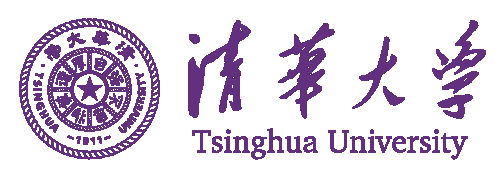
\includegraphics{thu-whole-logo}
  \caption{利用 Xfig 制图}
  \label{fig:xfig1}
\end{figure}

大学之道,在明明德,在亲民,在止于至善。知止而后有定;定而后能静;静而后能安;安
而后能虑;虑而后能得。物有本末,事有终始。知所先后,则近道矣。古之欲明明德于天
下者,先治其国;欲治其国者,先齐其家;欲齐其家者,先修其身;欲修其身者,先正其心;
欲正其心者,先诚其意;欲诚其意者,先致其知;致知在格物。物格而后知至;知至而后
意诚;意诚而后心正;心正而后身 修;身修而后家齐;家齐而后国治;国治而后天下
平。自天子以至于庶人,壹是皆以修身为本。其本乱而未治者 否矣。其所厚者薄,而其所
薄者厚,未之有也!

\hfill —— 《大学》


\subsubsection{多个图形}
\label{sec:multifig}

如果多个图形相互独立,并不共用一个图形计数器,那么
用 \texttt{minipage} 或者\texttt{parbox} 就可以。否则,请参看
图~\ref{fig:big1-subcaptionbox},它包含两个小图,分别是图~\ref{fig:subfig1}和
图~\ref{fig:subfig2}。推荐使用\cs{subcaptionbox},因为可以像
图~\ref{fig:big1-subcaptionbox} 那样对齐子图的标题,也可以使
用\pkg{subcaption}宏包的\cs{subcaption}(放在 minipage中,用法同\cs{caption})
或是 \pkg{subfigure} 、 \pkg{subtable}环境,像图~\ref{fig:big1-subfigure},
不要再用 \cs{subfloat}、\cs{subfigure} 和 \cs{subtable}。

\begin{figure}[h]
  \centering%
  \subcaptionbox{第一个小图形\label{fig:subfig1}}[3cm] %标题的长度,超过则会换行,如下一个小图。
    {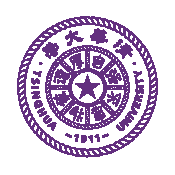
\includegraphics[height=3cm]{thu-fig-logo}}%
  \hspace{4em}%
  \subcaptionbox{第二个小图形,注意这个图略矮些。如果标题很长的话,它会自动换行\label{fig:subfig2}}
      {
\includegraphics[height=2cm]{thu-text-logo}}
  \caption{包含子图形的大图形(subcaptionbox示例)}
  \label{fig:big1-subcaptionbox}
\end{figure}
\begin{figure}[h]
  \centering%
  \begin{subfigure}{3cm}
    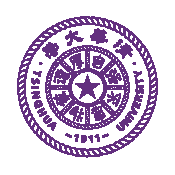
\includegraphics[height=3cm]{thu-fig-logo}
    \caption{第一个小图形}
  \end{subfigure}%
  \hspace{4em}%
  \begin{subfigure}{0.5\textwidth}
    
\includegraphics[height=2cm]{thu-text-logo}
    \caption{第二个小图形,注意这个图略矮些。subfigure中同一行的子图在顶端对齐。}
  \end{subfigure}
  \caption{包含子图形的大图形(subfigure示例)}
  \label{fig:big1-subfigure}
\end{figure}

古之学者必有师。师者,所以传道受业解惑也。人非生而知之者,孰能无惑?惑而不从师,
其为惑也,终不解矣。生乎吾前,其闻道也固先乎吾,吾从而师之;生乎吾後,其闻道也亦
先乎吾,吾从而师之。吾师道也,夫庸知其年之先後生於吾乎!是故无贵无贱无长无少,道
之所存,师之所存也。

嗟乎!师道之不传也久矣,欲人之无惑也难矣。古之圣人,其出人也远矣,犹且从师而问焉;
今之众人,其下圣人也亦远矣,而耻学於师。是故圣益圣,愚益愚。圣人之所以为圣,愚
人之所以为愚,其皆出於此乎?爱其子,择师而教之,於其身也,则耻师焉,惑焉。彼童子
之师,授之书而习其句读者,非吾所谓传其道、解其惑者也。句读之不知,惑之不解,或师
焉,或不焉,小学而大遗,吾未见其明也。巫医、乐师、百工之人不耻相师,  士大夫之族
曰“师”曰“弟子”之云者,则群聚而笑之。问之,则曰:彼与彼年相若也,道相似也,位
卑则足羞,官盛则近谀。呜呼!师道之不复,可知矣。巫医、乐师、百工之人。吾子不齿,
今其智乃反不能及,其可怪也欤!圣人无常师。孔子师郯子、苌子、师襄、老聃。郯子之徒,
其贤不及孔子。孔子曰:“三人行,必有我师。”是故弟子不必不如师,师不必贤於弟子。
闻道有先後,术业有专攻,如是而已。

如果要把编号的两个图形并排,那么小页就非常有用了:
\begin{figure}
\begin{minipage}{0.48\textwidth}
  \centering
  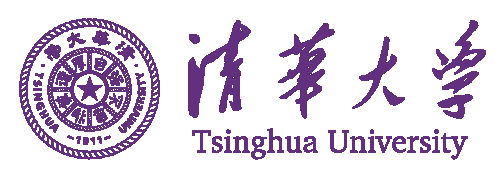
\includegraphics[height=2cm]{thu-whole-logo}
  \caption{并排第一个图}
  \label{fig:parallel1}
\end{minipage}\hfill
\begin{minipage}{0.48\textwidth}
  \centering
  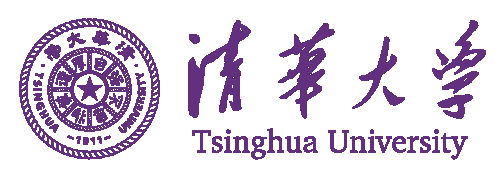
\includegraphics[height=2cm]{thu-whole-logo}
  \caption{并排第二个图}
  \label{fig:parallel2}
\end{minipage}
\end{figure}

李氏子蟠,年十七,好古文、六艺,经传皆通习之,不拘於时,学於余。余嘉其能行古
道,作师说以贻之。

\hfill —— 韩愈(唐)

 \chapter{绪论}
 % \documentclass{article}
 % \usepackage{ctex}
 % \usepackage{amsmath}
 % \begin{document}
 % \newtheorem{theorem}{定理}

\section{问题背景}
粘弹性流体广泛存在于日常生活中,粥、冰淇凌、油漆、细胞液等都是粘弹性流体。由于这些流体中存在高分子物质,它们表现出一定的弹性效应。流体在流动中同时表现出粘性和弹性的性质称为粘弹性。材料粘弹性行为的数学模型已经有很长的研究历史\cite{maxwell2013scientific,kelvin1887stability,oldroyd1950formulation,weissenberg1947continuum,zimm1956dynamics,ferry1980viscoelastic,larson1999structure} 。随着近些年来材料科学和生命科学的发展,越来越多的新材料被发现,例如液晶、凝胶、活性物质等\cite{de1975physics,prost2015active,marchetti2013hydrodynamics,ramaswamy2010mechanics,berthier2013non},并且对这些流体粘弹性性质的研究也获得了快速发展\cite{lin2012some,larson1999structure,joseph2013fluid}。

由于实际中的粘弹性流体大多是水溶液,目前大部分模型假设流体不可压缩。然而随着纳米科学等学科的发展,一些粘弹性流体的压缩性变得不可忽略\cite{yu2015compressible,galstyan2015note,chakraborty2015constitutive,pelton2009damping,kim1999numerical,lind2013bubble}。另外,目前大部分模型并没有考虑温度的影响,而实际上粘弹性流体的流动行为与温度密切相关。如何将流体的压缩性和温度纳入粘弹性流体的模型中,是一个具有挑战性的问题\cite{grmela1997dynamicsI,ottinger1997dynamicsII,larson1999structure}。

另外,由于粘弹性效应,粘弹性流体在热力学上处于非平衡态。经典平衡态热力学无法很好地对其进行描述。近些年来随着非平衡态热力学的发展,许多理论被应用于粘弹性流体的建模中\cite{jou1996extended,beris2013thermodynamics,ottinger2005beyond,coleman1961foundations,coleman1964thermodynamics,truesdell2012rational,truesdell2004non,eringen2012microcontinuum,eringen1965theory,zhu2014conservation}。然而,目前大多数理论是从物理原理出发,缺乏数学上对方程适定性的分析。如何建立一个既满足物理原理,又能够满足数学上要求的理论,对于粘弹性流体的数学建模具有重要意义\cite{zhu2014conservation,larson1999structure}。

本文的研究目的,就是推广Zhu、Hong、Yang、Yong提出的非平衡态热力学的守恒-耗散理论,为非等温可压粘弹性流体的建模提供新的手段。利用这些手段本文发展了几类非等温可压粘弹性流体模型并对其进行了数学分析。本文的结果,对于完善守恒-耗散理论、对于粘弹性流体的建模具有重要的意义,所提出的非等温可压粘弹性流体模型,完善了经典的不可压粘弹性流体力学理论。对模型的数学分析是对粘弹性流体进行数学上统一处理的一个尝试,并为粘弹性流体模型的数学分析提供了新的思路。

% 为了研究这些问题,本文考虑的粘弹性流体仅限于简单的高分子溶液。

\section{粘弹性流体建模的研究历程与现状}
对物质粘弹性建模的早期研究出现在19世纪下半叶,Maxwell从阻滞弹簧的模型出发提出了Maxwell线性粘弹性模型\cite{maxwell2013scientific}。经典的Maxwell模型方程如下
\begin{eqnarray*}
\frac {d\epsilon} {dt} = \frac {\sigma} {\eta} + \frac {1} {E} \frac {d\sigma} {dt},
\end{eqnarray*}
其中$\sigma$和$\epsilon$分别为材料的应力张量和应变张量,$\eta$和$E$分别为材料的粘性系数和弹性常数(模量)。在流体中$\frac {d\epsilon} {dt}$一般采用速度梯度量$\nabla v$的对称部分$D=\frac{1}{2} (\nabla v + (\nabla v)^T)$来代替,从而可以得到粘弹性流体的Maxwell模型如下
\begin{equation} \label{eq:maxwell}
			\partial_t \sigma + v \cdot \nabla \sigma - D = -\frac{\sigma}{\xi}. 
\end{equation}
交换上面方程中的应力应变张量得到的模型称为Kelvin-Voigt模型,由物理学家Kelvin和Voigt在19世纪末提出\cite{kelvin1887stability}。

19世纪中叶Weissenberg发现了Weissenberg效应。这一效应是指当转动的杆置于粘弹性流体中时,流体将会沿着杆“爬上”或者“爬下”\cite{weissenberg1947continuum}。为了解释这一效应,Oldroyd提出了粘弹性建模的重要法则:客观性原理。这一原理是说模型不应依赖于坐标系的选取。基于这一原理,他提出了客观导数的概念,并提出了经典的Oldroyd-B模型,这一模型如下
\begin{equation} \label{eq:Oldroyd}
	{\sigma} + \lambda_1 \stackrel{\nabla}{{\sigma}} = 2\eta_0 ({D} + \lambda_2 \stackrel{\nabla}{{D}}).
\end{equation}
其中$\sigma$为应力张量,$\lambda_1$和$\lambda_2$分别为松弛时间和迟滞时间,$\eta_0$为流体的粘性系数,${\stackrel{\nabla} \sigma}= \partial_t \sigma + v \cdot \nabla \sigma - (\nabla v)\  \sigma - \sigma (\nabla v)^T$为$\sigma$的上对流Maxwell导数\cite{oldroyd1950formulation}。Oldroyd的这一论文对粘弹性流体的建模产生了深远的影响。基于这一原理,修改经典Maxwell模型和Kelvin-Voigt模型中的导数为客观导数可以得到许多模型\cite{lin2005hydrodynamics,larson1999structure}。

我们一般将经典的Maxwell等不包含客观导数的模型称为线性粘弹性模型,而将Oldroyd-B等包含客观导数的模型称为非线性粘弹性模型。由上面的方法直接推广的非线性粘弹性模型仅能考虑简单的情况,不能很好地纳入温度的影响。为了解决这些问题,热力学家和力学家提出了许多理论,这些理论主要有两个方向:一是非平衡态热力学理论\cite{jou1996extended,ottinger2005beyond,zhu2014conservation},二是基于热力学原理和有限形变理论的记忆衰减理论\cite{coleman1961foundations,truesdell2012rational}。

\subsection{非平衡态热力学在粘弹性流体建模中的应用}
热力学第二定律告诉我们热力学体系非平衡状态的存在性。为了研究热力学不可逆过程,科学家发展了非平衡态热力学。Onsager在1931和1932年的两篇文章中提出了著名的Onsager倒易关系\cite{onsager1931reciprocal,onsager1931reciprocalII}。由Onsager与Prigogine等人发展的经典非平衡态热力学理论(Classical Irreversible Thermodynamics,简称CIT),自20世纪40年代以来获得了蓬勃发展,并且得到了广泛的承认\cite{jou1996extended,truesdell2012rational}。CIT理论可以将经典的Newton本构关系和Fourier热传导定律纳入其中,然而无法将Maxwell粘弹性模型和Cattaneo热传导模型纳入其理论框架中来。为了推广经典的CIT理论,许多新的非平衡态热力学理论被提出,其中包括理性热力学(Rational Thermodynamics,简称RT)、扩展不可逆热力学(Extended Irreversible Thermodynamics,简称EIT)、非平衡可逆-不可逆一般方程(General Equation for the Non-Equilibrium Reversible-Irreversible Coupling,简称GENERIC)、守恒-耗散理论(Conservation-Dissipation Formalism of irreversible thermodynamics,简称CDF)等\cite{truesdell2012rational,jou1996extended,ottinger2005beyond,zhu2014conservation}。

考虑一般的流体方程
\begin{subequations} \label{eq:fluid}
	\begin{align}
		\partial_t \rho + \nabla \cdot (\rho v) = 0 ,\\
		\partial_t (\rho v) + \nabla \cdot (\rho v \otimes v + P) =  0, \\
		\partial_t[\rho (u + \frac{1}{2} v^2)] + \nabla \cdot [q + \rho (u+\frac{1}{2}v^2) v + P \cdot v] = 0.
	\end{align}
\end{subequations}
其中$\rho,v,u$分别表示流体的密度、速度和内能,$P$表示流体的应力张量。这三个方程分别表示质量守恒、动量守恒和能量守恒。CIT假设平衡态的热力学状态参量仍然可以用来描述非平衡态,并且体系的熵依赖于这些状态变量。这里我们假设体系的比熵(单位质量的熵)为$s=s(\frac{1}{\rho},u)$,利用经典平衡态热力学的Gibbs关系,有
\begin{equation*}
	T ds = du + p d(\frac{1}{\rho}).
\end{equation*}
通过计算可以得到
\begin{equation*}
	\rho \dot{s} = - \frac{1}{T} \nabla \cdot q - \frac{1}{T} P: \nabla v,
\end{equation*}
其中$\dot{s} = \partial_t s + v \cdot \nabla s$表示物质导数。根据热力学第二定律,为保证不可逆过程熵函数的增长,需要$\rho \dot{s} \ge 0 $。根据Onsager倒易关系,热力学流和热力学力之间为线性关系。假设$P$可以分解为$P = p + \pi I + \mathring{P}$,其中$\mathring{P} = P - \frac{1}{3} \mbox{Tr}(P) I$为$P$的无迹部分。根据Onsager倒易关系,我们可以得到下面的本构关系
\begin{eqnarray*}
	q = -\lambda \nabla T, \\
	\pi =  - \zeta \nabla \cdot v, \\
	\mathring{P} = - 2 \eta \mathring{D}.
\end{eqnarray*}
此即热传导的Fourier定律与应力张量的Stokes和Newton本构关系

然而,由于局部平衡假设的存在,CIT仅能描述远离平衡态不远的系统。为了拓展CIT,大部分理论假设非平衡态的描述不仅需要平衡态变量,也需要非平衡态变量。Coleman、Truesdell、Noll等人发展了理性热力学RT。理性热力学理论认为非平衡态不仅依赖于平衡态状态变量,还依赖于状态变量的空间梯度。通过推广Clausius-Duhem不等式,利用Onsager倒易关系得到本构关系。Fourier-Stokes-Newton定律可以由RT理论导出\cite{jou1996extended}。另外,Jou、Lebon等人发展了扩展不可逆热力学EIT。EIT通过拓展非平衡态状态变量,将CIT中的热力学流引入非平衡态状态变量中,来对不可逆过程进行建模。例如我们将$q,\pi,\mathring{P}$引入非平衡态状态变量中,并假设$s = s(\frac{1}{\rho}, u,q,\pi,\mathring{P} )$,则通过计算可以得到熵的产生率为
\begin{equation*}
		\rho \dot{s} = - \frac{1}{T} \nabla \cdot q - \frac{1}{T} P: \nabla v - \alpha_1 \pi \cdot \dot{\pi} - \alpha_2 q \cdot \dot{q} - \alpha_3 \mathring{P} : ({\mathring{P} })^. ,
\end{equation*}
其中$\alpha_1,\alpha_2,\alpha_3$为常数。EIT仍然假设Onsager倒易关系成立,利用Onsager关系,可以得到下面的本构关系。
\begin{subequations} \label{eq:EITconstitutive}
		\begin{align}
	\nabla T^{-1} - \alpha_2 \dot{q} = \mu_1 q - \beta^{''}\nabla \cdot \mathring{P} - \beta' \nabla \pi, \\
	-T^{-1} \nabla \cdot v - \alpha_1 \dot{\pi} = \mu_0 \pi - \beta' \nabla \cdot q , \\
	-T^{-1} \mathring{D} - \alpha_3 (\mathring{P})^. = \mu_2 \mathring{P} - \beta^{''} (\mathring{\nabla q})^s,
		\end{align}
\end{subequations}
其中$A^s = \frac{1}{2} (A+A^T)$表示张量$A$的对称部分。通过取合适的参数可以得到Maxwell-Cattaneo定律。
\begin{eqnarray*}
	\tau_1 \dot{q} + q = - \lambda \nabla T, \\
 	\tau_0 \dot{\pi } + \pi = -\zeta \nabla \cdot v, \\
 	\tau_2 (\mathring{P})^. + \mathring{P} = -2 \eta \mathring{D}.
\end{eqnarray*}
其中$\sigma = \pi I + \mathring{P}$。对于不可压流体,我们可以得到Maxwell模型。EIT可以很好地用于线性粘弹性流体模型,然而对于含客观导数的非线性粘弹性本构关系,缺乏简单的处理方式\cite{jou1996extended}。

为了处理复杂的非线性粘弹性流体模型,Beris和Edwards等人通过拓展经典力学的Hamilton理论,在Possion括号之外引入耗散括号(dissipative bracket)来描述能量的耗散和不可逆过程熵的增长\cite{edwards1990remarks,beris2013thermodynamics}。假设$X$为非平衡态系统的状态变量,系统的广义Hamilton函数设为$H=H(X)$,则$X$的演化方程为
\begin{equation*}
	\frac{dX}{dt} = L(X) \cdot \frac{\delta H(X)}{\delta X} + M(X) \cdot \frac{\delta H(X)}{\delta X}, 
\end{equation*}
其中$L=L(x)$和$M=M(x)$为体系的Possion矩阵和耗散矩阵。这一理论通过给出系统的能量和熵函数,并选取合适的$L$和$M$而得到描述体系的方程。 为了满足能量守恒和熵增原理,我们假设$L$与$M$可以定义Possion括号和耗散括号
\begin{equation*}
	\{ A,B \} = \frac{\delta A(X)}{\delta X} \cdot L(X) \cdot \frac{\delta B(X)}{\delta X}, \quad  [ A,B ] = \frac{\delta A(X)}{\delta X} \cdot M(X) \cdot \frac{\delta B(X)}{\delta X}. 
\end{equation*}
其中$L$的选取需要满足经典的Possion括号定义,$M$的选取使得下面的条件成立
\begin{equation*}
	[\int \rho(x) dx, H]=0,[\int \rho(x) v(x) dx, H]=0, \quad [E,H] = 0,
\end{equation*}
以及
\begin{equation*}
	[S,H] \ge 0,
\end{equation*}
由此可知守恒率和热力学第二定律成立。对于不可压粘弹性流体,我们忽略温度的影响,则可以取状态变量$X= 
 \{v,c\}$,其中张量$c$表示非平衡态变量(与粘弹性引起的应变能耗散有关)。取Hamilton量为
 \begin{equation*}
 	H = \int \frac{1}{2} v^2(x) + \frac{1}{2} \mbox{
 	Tr}(c(x))- \frac{1}{2}  \ln \det c(x) dx,
 \end{equation*}
以及Possion矩阵和耗散矩阵为
\begin{equation*}
	L = \left( \begin{array}{cc} 
			u \cdot \nabla &  L_{12} \\
			L_{21}& 0
		\end{array}\right), \quad
	M =	\left( \begin{array}{cc} 
			0  & 0 \\
			0  & c \otimes I
		\end{array}\right),
\end{equation*}
其中
\begin{eqnarray*}
	(L_{12})_{l,kj} = - \frac{\partial}{\partial x_m} c_{mk} \delta_{jl} -  \frac{\partial}{\partial x_m} c_{jm} \delta_{kl}, \\
	(L_{21})_{jk,l} = -c_{mk} \delta_{jl} \frac{\partial}{\partial x_m} - c_{jm} \delta_{kl} \frac{\partial}{\partial x_m}.
\end{eqnarray*}
这里$m$对$1$到$n$求和,$n$为空间维数。本文中如无特别说明,我们采用Einstein求和约定,相同的指标表示求和。
取能量和熵函数为
\begin{equation*}
	E = \int \frac{1}{2} v^2(x)dx, \quad S = -\int \frac{1}{2} \mbox{
 	Tr}(c(x))- \frac{1}{2}  \ln \det c(x) dx.
\end{equation*}
我们可以得到下面的上对流Maxwell模型
\begin{subequations}\label{eq:chap1UCMmaxll}
\begin{align}
	v_t + v \cdot \nabla v + \nabla p  - \nabla \cdot (c - I) = 0, \\
	c_t + v \cdot \nabla c - (\nabla v)c - c (\nabla v)^T = -\frac{c-I}{\lambda}.
\end{align}
\end{subequations}

由于Beris和Edwards理论对耗散括号要求的复杂性,如何提出满足要求的耗散矩阵是一个很有挑战性的问题。为了解决这一问题,\"Ottinger与Grmela发展了GENERIC理论\cite{ottinger2005beyond}。GENERIC并不假设非平衡态Hamilton函数的存在,而是仅仅假设能量和熵的存在性。假设$X$为非平衡态系统的状态变量,其演化方程可以写为
\begin{equation*}
	\frac{dX}{dt} = L(X) \cdot \frac{\delta E(X)}{\delta X} + M(X) \cdot \frac{\delta S(X)}{\delta X} ,
\end{equation*}
其中$E=E(X)$和$S=S(X)$分别为系统的能量和熵,$L=L(x)$和$M=M(x)$为体系的Possion矩阵和耗散矩阵。GENERIC通过给出系统的能量和熵函数,选取合适的$L$和$M$即可得到描述体系的方程。 为了满足能量守恒和熵增原理,我们假设$L$与$M$可以定义Possion括号和耗散括号
\begin{equation*}
	\{ A,B \} = \frac{\delta A(X)}{\delta X} \cdot L(X) \cdot \frac{\delta B(X)}{\delta X}, \quad  [ A,B ] = \frac{\delta A(X)}{\delta X} \cdot M(X) \cdot \frac{\delta B(X)}{\delta X}. 
\end{equation*}
其中$L$的选取需要满足经典的Possion括号定义,$M$的选取使得下面的条件成立
\begin{equation*}
	[A,B] = [B,A], \quad [A,A] \ge 0.
\end{equation*}
假设系统的能量为$E$,熵函数为$S$,我们假设$L,M$满足下面的退化条件
\begin{equation}
	L \frac{\delta S}{\delta X} = 0, \quad M \frac{\delta E}{\delta X} = 0,
\end{equation}
那么任意泛函$A$的演化方程为
 \begin{equation*}
	\frac{d A}{dt} = \frac{\delta A(x)}{\delta x} \cdot \frac{dx}{dt} = \{ A,E\} + [A,S].
\end{equation*}
于是可以得到
\begin{eqnarray*}
	\frac{d E}{dt} = \{E,E\} +[S,E] = 0, \\
	\frac{d S}{dt} = [S,S] \ge 0. 
\end{eqnarray*}
这里我们用到了退化条件$[E,S] = 0$。在GENERIC中关键的是选取合适的Possion矩阵和耗散矩阵,使之满足Possion括号和耗散括号的定义以及退化条件。GENERIC将物理量的演化分成了两个部分,一部分是由可逆过程引起的,而另一部分是由不可逆过程引起的,具体通过Possion括号和耗散括号实现,并且与退化条件一起保证了热力学第一定律和第二定律的成立。然而在上面上对流Maxwell模型的例子中,却很难将可逆过程和不可逆过程的影响通过这种方式分开,如果我们采用上面的能量和熵函数$E,S$,以及矩阵$L,M$,那么可以验证$L$不满足退化条件。  

由于EIT缺乏对含客观导数的非线性粘弹性模型的考虑,Beris-Edwards中Possion矩阵和耗散矩阵选取的复杂性以及GENERIC对可逆部分和不可逆部分耦合方式的简单性,这些理论都没有完美地解决粘弹性流体的建模问题。另一方面,这些理论建立在物理定律的基础上,缺乏对方程数学性质的分析。除上面提到的非平衡态热力学理论之外,也有很多其他的非平衡态热力学理论试图解决粘弹性流体的建模问题,可以参看\cite{stratonovich2012nonlinear,huo1993nonequilibrium,eu1992kinetic}。

基于Yong的双曲方程守恒-耗散结构条件\cite{yong2008interesting},Zhu、Hong、Yang、Yong发展了不可逆热力学的守恒-耗散理论(CDF)\cite{zhu2014conservation}。Yong等发展的守恒-耗散理论(以下简称守恒-耗散理论)通过守恒-耗散结构条件保证了热力学第一定律和第二定律的成立,并且得到的方程组满足Yong的稳定性条件,从而有着良好的数学性质\cite{yong1992singular}。守恒-耗散理论已经顺利地应用于线性粘弹性流体力学模型\cite{zhu2014conservation}。然而,由于目前的守恒-耗散理论考虑的是守恒形式的方程,而客观导数的存在将会导致方程不再可以写成守恒形式,所以守恒-耗散理论在应用到非线性粘弹性流体模型时遇到了困难。本文将推广这一理论并将其应用于非线性粘弹性流体的建模中。

\subsection{粘弹性流体的记忆衰减理论}
由于粘弹性流体可以看作连续介质,所以可以采用连续介质力学的理论对其进行建模。前文提到的模型一般都是通过小变形连续介质力学得到的,而对于粘弹性流体来说,尤其是高弹性的流体,小形变假设不再适用。基于此,Coleman和Noll等人提出了利用有限形变理论对粘弹性流体进行建模的方法\cite{coleman1961foundations,coleman1964thermodynamics,coleman2012viscometric}。该理论认为物质的状态依赖于其形变的历史,而形变可以用形变张量$F$来描述。这里$F$定义为流动图$x = x(X,t)$的梯度$F_{ij} = \frac{\partial x_i}{\partial X_j}$,其中$x,X$分别对应于流体质点的Euler和Lagrange坐标。根据定义可以得到
\begin{equation}\label{eq:Feq}
	\partial_t F + v \cdot \nabla F = (\nabla v) F.
\end{equation}
这一理论认为应力张量是$F$的历史和温度$\theta$的历史的函数。假设体系的自由能为
\begin{equation*}
	\psi = \mathop{\psi} \limits_{\tau=0}^{t}( C(t), C^t(\tau),\theta(t),\theta^t(\tau)).
\end{equation*}
其中$C(t) = F^T(t) F(t),C^t(\tau) = C(t - \tau)$。$\psi$依赖于从初始时刻到当前时刻$t$的应变历史。利用Gibbs关系,可以得到
\begin{equation}\label{eq:en}
	\rho \frac{d\psi}{dt} + \rho \eta \frac{d \theta}{dt} - T: \frac{dC}{dt} + w = 0.
\end{equation}
其中$T$代表第二Piola-Kirchhoff张量,与Cauchy应力张量$\sigma$的关系为$\sigma = \rho F T F^T$,$w$代表能量的耗散。由$\psi$的表达式可以得到
\begin{equation*}
	\frac{d\psi}{dt} = \frac{\partial \psi}{\partial C} : \frac{d C}{dt}+ \frac{\partial \psi}{\partial \theta} \frac{d\theta}{dt} + \delta \psi.
\end{equation*}
代入\eqref{eq:en}中得到
\begin{equation*}
	(\rho \frac{\partial \psi}{\partial C} - T) : \frac{dC}{dt} + \rho (\frac{\partial \psi}{\partial \theta} + \eta) d\theta + (w + \rho \delta \psi) dt  =0.
\end{equation*}
从而得到
\begin{eqnarray*}
	T = \rho \frac{\partial \psi}{\partial C} = \mathop{\mathcal{F}}\limits_{\tau=0}^{t} ( C(t), C^t(\tau),\theta(t),\theta^t(\tau)), \\
	\eta = -\frac{\partial \psi}{\partial \theta},\\
	w = -\rho \delta \psi.
\end{eqnarray*}
热力学第二定律由$w \ge 0$保证\cite{coleman1961foundations,dimitrienko2010nonlinear}。

例如经典的上对流Maxwell模型的熵函数可以取作(忽略温度)
\begin{equation*}
	\psi  = \psi(t) = - \frac{1}{\lambda}  \ln \det (F^T(t) F(t)) + F^T(t) F(t) : \frac{1}{\lambda}  \int_{0}^t e^{-\frac{t-s}{\tau}} F^{-1}(\tau) F^{-T}(\tau) d\tau,
\end{equation*}
于是有
\begin{equation*}
	T = \frac{1}{\lambda}  \int_{0}^t e^{-\frac{t-s}{\tau}} F^{-1}(\tau) F^{-T}(\tau) d\tau -\frac{1}{\lambda}  F^{-1} F^{-T} .
\end{equation*}
应力张量$\sigma$可以写为
\begin{equation*}
	\sigma = \frac{1}{\lambda} \int_{0}^{t} e^{-\frac{(t-s)}{\lambda} } F(t)  F^{-1}(s) F^{-T}(s) F^T(t)  dx.
\end{equation*}
注意上面的积分是沿流线的积分。于是根据\eqref{eq:Feq},可以得出$\sigma$满足上对流Maxwell模型,该模型的能量耗散为
\begin{equation*}
	w = - \rho \frac{1}{\lambda} \mbox{Tr}(I) = -\frac{3\rho}{\lambda} < 0.
\end{equation*}
这违背了热力学第二定律对$w>0$的要求。所以这一理论不能很好地包括上对流Maxwell模型。


另外,Lin、Liu、Zhang在文献\cite{lin2005hydrodynamics}中提出了下面的模型
\begin{subequations}\label{eq:linincompressible}
	\begin{align}
		\nabla \cdot v = 0, \\
		v_t + v \cdot \nabla v + \nabla p = \mu \Delta v + \nabla \cdot( F F^T), \\
		F_t + v \cdot \nabla F = \nabla v F.
	\end{align}
\end{subequations}
Lei、Liu、Zhou在\cite{lei2008global}中发展这一方程组至可压缩形式。可压形式的方程组如下
\begin{subequations}\label{eq:lincompressible}
	\begin{align}
		\rho_t + \nabla \cdot (\rho v) = 0, \\
		(\rho v)_t + \nabla \cdot (\rho v \otimes v) + \nabla p = \mu \Delta v + \mu' \nabla \nabla \cdot v+ \nabla \cdot( \rho F F^T), \\
		F_t + v \cdot \nabla F = \nabla v F.
	\end{align}
\end{subequations}
这一模型实际上对应于无穷大Weissenberg数Oldroyd模型\cite{lei2008global},以下简称这一模型为Lin等人的模型。这里的模型实际上是Navier-Stokes方程的一个推广,利用有限形变理论将弹性形变$\rho F F^T$包含在了应力张量之中。这一模型因为有着良好的数学结构而得到了许多数学上好的结果\cite{lin2012some},但是尚缺乏在实际中的应用实例。

综上所述,有限形变理论是一个描述连续介质力学的很好工具。利用有限形变理论,结合非平衡态热力学的方法发展起来的热力学理论在粘弹性流体的建模方面有一定的优势,但是也存在一些问题。

本论文将讨论基于守恒-耗散理论和有限形变理论的粘弹性流体建模方法。

\section{粘弹性流体的数学分析}
由于粘弹性流体方程的重要性和复杂性,其数学分析一直以来都吸引了很多数学家的兴趣\cite{lin2012some,li2007mathematical,weinan2002convergence,fabrizio1992mathematical,renardy2008mathematical,joseph1987hyperbolicity,guillope2010regular,saut2012lectures,yong2014newtonian,qian2010well,hu2011global,lei2005global,fang2014incompressible}。目前的分析主要集中于不可压方程,主要包括Oldroyd-B模型、上对流Maxwell模型、FENE模型、以及Lin等人的模型\cite{elgindi2015global,saut2012lectures,renardy2000mathematical,masmoudi2011global,lions2000global,masmoudi2008well,lei2010remarks}。近些年来,也有部分工作讨论了可压粘弹性流体方程\cite{fang2014incompressible,hu2012strong,qian2010global,qian2011initial}。
\subsection{经典粘弹性流体力学模型的数学分析}
经典的粘弹性流体模型主要包括线性粘弹性流体力学模型Maxwell模型\eqref{eq:maxwell}和Kelvin-Voigt模型,以及非线性粘弹性流体模型上对流Maxwell模型\eqref{eq:chap1UCMmaxll}、Oldroyd-B模型\eqref{eq:Oldroyd}和采用其他客观导数的类似模型等。对这些方程的分析主要集中于方程弱解的全局存在性、光滑解的局部存在性、平衡态附近解的整体存在性,以及松弛参数(通常为Weissenberg数)趋于$0$时的极限分析。我们这里只考虑宏观模型,对于微观模型的数学结果可以参看Masmoudi、Li、Zhang、E、Sun等人的工作\cite{masmoudi2013global,masmoudi2008well,li2007mathematical,li2004local,li2004well,lions2007global,weinan2002convergence,constantin2010remarks}。

对于线性粘弹性流体的分析结果可以参看\cite{fabrizio1992mathematical,renardy2000mathematical}。书中对线性粘弹性的数学结果做了总结,主要讨论并证明了方程解的存在性和唯一性、稳定性和稳态方程解的存在性和唯一性。由于线性粘弹性流体的适用范围的局限性,大部分分析工作均围绕非线性粘弹性流体模型。最简单的非线性粘弹性流体模型是对流导数Maxwell模型和Oldroyd模型。首先我们考虑对流导数的Maxwell模型
\begin{subequations}\label{eq:Oldroyda}
\begin{align}
	\lambda \frac{\mathcal{D}_a \sigma}{\mathcal{D} t} + \sigma = 2 \eta D, \\
	\partial_t v + v \cdot \nabla v  + \nabla p = \nabla \cdot \sigma, \\
	\nabla \cdot v = 0,
\end{align}
\end{subequations}
其中
\begin{equation*}%\label{eq:convectderivative}
	\frac{\mathcal{D}_a \sigma}{\mathcal{D} t} = \partial_t \sigma + v \cdot \nabla \sigma + \sigma W- W \sigma - a(D \sigma + \sigma D), \ W = \frac{1}{2}(\nabla v - (\nabla v)^T).
\end{equation*}
当$a=1$时\eqref{eq:Oldroyda}为上对流Maxwell模型\eqref{eq:chap1UCMmaxll},$a=-1,0$分别对应于Jaumann和下对流导数Maxwell模型。针对方程组\eqref{eq:Oldroyda},Rutkevich等人对其双曲性进行了分析\cite{rutkevich1969some,rutkevich1970propagation},Joseph、Saut、Renardy等人发展了Rutkevich的结果\cite{joseph1987hyperbolicity,joseph1986change}。由这些工作,可以得到方程组\eqref{eq:Oldroyda}在下面的条件下会出现Hadamard不稳定性:
\begin{equation*}
	\frac{1-a}{2} \Lambda_M - \frac{1+a}{2} \Lambda_m > \frac{\eta}{\lambda}.
\end{equation*}
其中$\Lambda_M$和$\Lambda_m$分别为$\sigma$的最大和最小特征值。根据这一分析,可以得到不稳定性仅可能在$a\in (-1,1)$时发生。对于上对流和下对流导数(分别对应于$a=-1$和$1$),模型\eqref{eq:Oldroyda}是双曲的,不会出现Hadamard不稳定性。
% 另外Joseph、Saut、Renardy等人还对稳态方程的双曲性进行了分析。
另外对该模型解的存在性结果可以参看\cite{saut2012lectures}。

由于Oldroyd模型的广泛应用和重要性,大部分数学工作都是围绕这一方程进行的。这一模型的一般方程为
\begin{subequations}\label{eq:Oldroydb}
\begin{align}
	\lambda \frac{\mathcal{D}_a \sigma}{\mathcal{D} t} + \sigma = 2 \eta_p D, \\
	\partial_t v + v \cdot \nabla v  + \nabla p = \nabla \cdot \sigma + 2 \eta_s \Delta v, \\
	\nabla \cdot v = 0.
\end{align}
\end{subequations}
其中$\eta_s,\eta_p$分别为溶剂和溶质的粘性系数。这一模型与对流导数Maxwell模型\eqref{eq:Oldroyda}的区别是在动量方程中添加了溶剂粘性$2\eta_s \Delta v$一项。
下面我们将讨论这一模型的主要数学结果。首先其解的局部存在性定理由Guillope、Saut等人在\cite{guillope1990existence}给出。证明主要采用了包含时间的Stokes问题的解的存在性结果\cite{temam1995navier},并利用了Sobolev演算不等式\cite{majda2012compressible}和经典的不动点理论。例如对于\eqref{eq:Oldroydb}中$\sigma$的估计,$\sigma$的方程两端与$\sigma$做内积可以得到
\begin{equation*}
	\frac{d}{dt} \|\sigma\|_{L^2}^2  =  -\frac{1}{\lambda} \|\sigma\|_{L^2}^2 + 2 (\frac{\eta}{\lambda} D, \sigma) + \left( (a(D \sigma + \sigma D) - (\sigma W -W \sigma)),\sigma \right).
\end{equation*}
右端第二项可以利用H\"older不等式估计如下
\begin{equation*}
	(\frac{\eta}{\lambda} D, \sigma) \le \frac{\eta}{\lambda} \|\sigma\|_{L^2} \|\nabla v\|_{L^2}.
\end{equation*}
第三项可以估计为
\begin{equation*}
	 \left( (a(D \sigma + \sigma D) - (\sigma W -W \sigma)),\sigma \right) 
%\le \|\sigma\|_{L^2}^2 \|\nabla v\|_{L^\infty} 
\le \|\sigma\|^2_{L^2} \|\nabla v\|_{H^2}
.
\end{equation*}
上式中最后一个不等号由Sobolev嵌入定理得到。为了估计$\|\nabla v\|_{H^2}$,需要对$v$的方程估计,最终可以得到\cite{guillope1990existence}
\begin{equation*}
		\frac{d}{dt} \|\sigma\|_{H^2}^2 + \frac{1}{\lambda} \|\sigma\|_{H^2}^2 \le C \frac{\eta}{\lambda} \|v\|_{H^3} \|\sigma\|_{H^2} + C \|v\|_{H^3} \|\sigma\|_{H^2}^2.
\end{equation*}
从而得到$\sigma \in L^\infty([0,T],H^2)$。然后利用Stokes问题的结论,最终可以证明下面的局部存在性定理:
\begin{theorem}(Guillope,Saut等\cite{guillope1990existence,saut2012lectures})
	假设$\sigma_0 \in H^2(\mathbf{R}^3),v_0 \in D(A)$,$D(A)$为$L^2$上Stokes算子的定义域。那么存在时间$T>0$,使得方程组\eqref{eq:Oldroydb}存在唯一的光滑解$(v,p,\sigma)$,且满足
	\begin{equation*}
		v \in L^2([0,T],H^3) \cap C([0,T],D(A)), \ p \in L^2([0,T],H^2) \ \sigma \in C([0,T],H^2).
	\end{equation*}
\end{theorem}
方程\eqref{eq:Oldroydb}的平衡点$(v=0,\sigma=0)$附近解的整体存在性首先由文献\cite{guillope1990existence}给出,其中假设了$\eta_s/\eta_p$足够大。这一假设是为了保证粘性项$ 2 \eta_s \Delta v$的耗散足够好从而使得$\sigma$的范数可以被$v$的范数控制。采用不同的方法,这一假设被移除,更一般的整体存在性结果也已经被证明\cite{chupin2004some,molinet2004global,molinet2004existence}。Molinet等人采用了$\|\mathcal{P}\nabla \cdot \sigma\|_{H^1}$来代替文献\cite{guillope1990existence}中的$\|\nabla \cdot \sigma\|_{H^1}$估计,从而得到更好的结果如下\cite{molinet2004global,molinet2004existence}:
\begin{theorem}(Molinet等\cite{molinet2004existence})
	假设$\sigma_0 \in H^2(\mathbf{R}^3),v_0 \in D(A)$足够小,那么方程组\eqref{eq:Oldroydb}在$t\in [0,\infty)$上存在唯一的光滑解$(v,p,\sigma)$,且满足
	\begin{eqnarray*}
		v \in L^2([0,\infty],H^3) \cap C([0,\infty],D(A)), \ p \in L^2([0,\infty],H^2), \ \sigma \in C([0,\infty],H^2).
	\end{eqnarray*}
\end{theorem}

在$L^p$框架下方程组\eqref{eq:Oldroydb}解的存在性证明可以参见Fernandez、Zhang和Fang的工作\cite{fernandez1998some,zhang2012global}。Besov空间的存在性结果见Chemin和Masmoudi的工作\cite{chemin2001lifespan}。

对于方程组\eqref{eq:Oldroydb}的弱解的整体存在性,Constantin和Sun证明了空间$C^\alpha(\mathbf{R}^n) \cap L^1(\mathbf{R}^n)$中弱解的存在性\cite{constantin2010remarks,saut2012lectures}。对于$a=0$的情况,$L^2$意义下弱解的整体存在性被Lions和Masmoudi证明\cite{lions2000global}。这一证明利用了对于$a=0$的模型,方程组\eqref{eq:Oldroydb}中$\sigma$成立下面的估计
\begin{equation*}
	\frac{d}{dt} \left(\frac{1}{2} \|v\|_{L^2}^2 +  \frac{\lambda}{4 \eta_p} \|\sigma\|_{L^2}^2 \right) + \frac{1}{2\eta_p} \|\sigma\|_{L^2}^2 + {2 \eta_s} \|\nabla v\|_{L^2}^2 = 0,
\end{equation*}
然而由于对于一般的情况,这一估计并不成立,弱解的存在性也尚未得到证明\cite{saut2012lectures}。

另外一个重要的数学问题为$\lambda$趋于$0$时方程组\eqref{eq:Oldroydb}的极限分析。形式上$\lambda$为$0$时我们得到Navier-Stokes方程组,即Newton流体模型。这一问题也经常被称为Newton极限问题。我们将$\sigma$的方程写成下面的形式
\begin{equation*}
	 \sigma = -	\lambda \frac{\mathcal{D}_a \sigma}{\mathcal{D} t} +  2 \eta_p D.
\end{equation*}
$\lambda=0$时,$\sigma= 2 \eta_p D$,从而方程组\eqref{eq:Oldroydb}成为经典的不可压Navier-Stokes方程组:
\begin{subequations} \label{eq:innavierstokes}
\begin{align}
	\partial_t v + v \cdot \nabla v  + \nabla p &= \nabla \cdot \sigma + 2 \eta \Delta v, \\
	\nabla \cdot v &= 0.
\end{align}
\end{subequations}
其中$\eta= \eta_s + \eta_p$。Molinet和Talhouk基于Fourier分析,通过对低频和高频情况的分析,得到了\eqref{eq:Oldroydb}和上面的Navier-Stokes方程组\eqref{eq:innavierstokes}兼容性的分析。证明了下面的定理:
\begin{theorem}(Monlinet和Talhouk\cite{molinet2008newtonian})
	令$n=2,3$,$(v_0,\sigma_0) \in H^s(\mathbf{R}^n) \times H^s(\mathbf{R}^{n^2}), s>\frac{n}{2}$。假设$v$为方程组\eqref{eq:innavierstokes}以$v_0$为初值的解,在$[0,T_0],T_0>0$上存在且$v \in C([0,T_0],H^s)$。那么对于任意的$\delta \in (0,1)$,存在
	\begin{equation*}
		\varepsilon_0 = \varepsilon_0 (n,\lambda,\eta_p,\eta_s,\delta, \|v\|_{{L_{T_0}^\infty}H^s}, \|\nabla v\|_{{L^2_{T_0}}H^s}, \|\sigma_0\|_{H^s}) >0,
	\end{equation*}
	使得对任意的$0 < \lambda < \varepsilon_0$,满足$0 < \frac{\eta_p}{\eta} \le 1- \delta$的方程组\eqref{eq:Oldroydb}存在唯一解
	\begin{equation*}
		v_\lambda \in C([0,T_0],H^s),\ \nabla v_{\lambda} \in L^2([0,T_0],H^s), \ \sigma_{\lambda} \in C ([0,T_0],H^s),
	\end{equation*}
	且当$\lambda \rightarrow 0$时,成立
	\begin{eqnarray*}
		v_\lambda \rightarrow v \quad \text{在} C([0,T_0],H^s) \text{中}, \\ 
		\sigma_\lambda - 2\eta_p D[v_\lambda]  \rightarrow v \quad \text{在} L^2([0,T_0],H^s) \text{中}, \\ 
		\lambda^{\frac{1}{2}} \sigma_\lambda \rightarrow v \quad \text{在} C([0,T_0],H^s) \text{中}.
	\end{eqnarray*}
\end{theorem}
这样对于$\eta_s \neq 0, \eta_p \neq 0$的情况,方程组\eqref{eq:Oldroydb}和Navier-Stokes方程组\eqref{eq:innavierstokes}的兼容性得到了严格地分析。另外,对于弱解下的Newton极限的分析,可以参看\cite{bresch2014newtonian}。


近些年来,一些可压缩粘弹性流体力学模型的数学分析开始吸引一些数学家的兴趣,主要集中于推广的Oldroyd模型。Bollada和Phillips总结了关于可压粘弹性模型的数学建模工作\cite{bollada2012mathematical},并利用Lie导数和微分几何导出了可压上对流Maxwell模型。关于这些模型的分析工作目前主要集中于局部存在性和平衡态附近的整体存在性的证明以及不可压极限的分析\cite{zhang2012global,fang2013strong,fang2014incompressible,matuvsuu1999existence,fang2013strong,barrett2016existence,salloum2011local}。例如,Fang和Zi等\cite{fang2013strong}给出了下面的可压Oldroyd-B模型
\begin{subequations}
	\begin{align*}
	\rho_t + \nabla \cdot (\rho v) = 0. \\
	(\rho v)_t + \nabla \cdot (\rho v \otimes v)  + \nabla p = \nabla \cdot \sigma + 2 \eta_s \Delta v, \\
	\lambda \frac{\mathcal{D}_a \sigma}{\mathcal{D} t} + \sigma = 2 \eta_p D
	\end{align*}
\end{subequations}
的局部存在性结果。其不可压极限为\eqref{eq:Oldroydb}的分析在\cite{fang2014incompressible}给出。

另外,也有许多关于其他模型的数学分析工作,例如FENE模型\cite{masmoudi2008well,zhang2006local,jourdain2004existence,liu2008boundary}、Giesekus模型\cite{renardy1984existence}等等。

\subsection{Lin等人的模型的数学分析}
由于Lin等人的模型有着良好的数学结构,其吸引了许多数学家的兴趣\cite{lin2005hydrodynamics,lebon2008classical,qian2010well,qian2011initial,hu2012formation,hu2015global}。在\cite{lin2005hydrodynamics}中,该方程在二维的Cauchy问题的局部存在性和在平衡态附近的整体存在性均得到了证明。证明基于力学上的适应性条件$\nabla \cdot F^T=0$,由此可以找到势函数$\phi$,使得$F = \nabla \times \phi$,在二维时
\begin{equation*}
	F = \left( \begin{matrix}
		-\partial_{x_2} \phi_1 & -\partial_{x_2} \phi_2 \\
		\partial_{x_1} \phi_1 & \partial_{x_1} \phi_2
	\end{matrix}\right).
\end{equation*}
于是方程组\eqref{eq:linincompressible}可以写为下面的形式
\begin{eqnarray*}
	\nabla \cdot v = 0, \\
	v_t + v \cdot \nabla v + \nabla p =  \mu \Delta v - \sum_{i=1}^2 \Delta \phi_i \nabla \phi_i, \\
	\phi_t + v \cdot \nabla \phi = 0.
\end{eqnarray*}
利用Galerkin逼近,其解的局部存在性可以得到证明\cite{lin2005hydrodynamics},证明过程采用了Gagliardo–Nirenberg插值不等式
\begin{equation*}
	\|v\|_{L^4}^2 \le C \|v\|_{L^2} \| \nabla v\|_{L^2} ,\ \|\nabla \phi\|_{L^4}^2 \le C \|\nabla \phi\|_{L^2}^{3/2} \|\nabla \Delta \phi\|_{L^2}^{1/2}.
\end{equation*}
利用基本的能量估计和上面的不等式,对高阶导数进行估计,可以得到下面的存在性定理:
\begin{theorem}(Lin、Liu、Zhang\cite{lin2005hydrodynamics})
	令$s \ge 2$,$\nabla \phi_0 \in H^s(\mathbf{R}^2),v_0 \in H^s(\mathbf{R}^2)$。那么存在仅仅依赖于$\|\nabla \phi_0\|_{H^2}$和$\|v_0\|_{H^2}$的时间$T>0$,使得方程\eqref{eq:linincompressible}在时间区间$[0,T]$上存在唯一解$U=(v,F=\nabla \phi) \in C([0,T],H^s) \cap C([0,T],H^{s+1})$。且如果解的最大存在时间为$T^*$,那么
	\begin{equation*}
		\int_0^{T^*} \|\nabla v\|_{H^2}^2 ds = + \infty.
	\end{equation*}
\end{theorem}

为了分析方程\eqref{eq:linincompressible}在二维时解在平衡态附近的整体存在性。取$\psi(x) = \phi(x)-x$,并令$w=v-\frac{1}{\mu}\psi$,而将方程组\eqref{eq:linincompressible}写成下面的形式
\begin{eqnarray*}
	\nabla \cdot v =0 , \\
	w_t - \mu \Delta w = - v \cdot \nabla w - \nabla p = - \Delta \psi \nabla \psi + \frac{v}{\mu}, \\
	\psi_t + v \cdot \nabla \psi = -v.
\end{eqnarray*}
这样一来在平衡态附近$w$由于右端项$-v$的衰减效应,以及$w$方程的抛物效应,该方程的整体解存在,下面的定理成立:
\begin{theorem}(Lin、Liu、Zhang\cite{lin2005hydrodynamics})
	令$s \ge 2$,$\nabla \phi_0 \in H^s(\mathbf{R}^2),\det(\phi_0) = 1, v_0 \in H^s(\mathbf{R}^2)$。那么对于足够小的$\|\nabla \psi_0\|_{H^2}$和$\|v_0\|_{H^2}$,方程\eqref{eq:linincompressible}存在唯一的整体光滑解$U=(v,F-I=\nabla \psi) \in C([0,\infty],H^s)$,且满足
	\begin{equation*}
		\|v\|_{H^2}^2 +\|\nabla \psi\|_{H^2}^2 + \int_0^\infty \|\nabla v\|_{H^2}
^2ds \le C \|\nabla \psi_0\|_{H^2} + \|v_0\|_{H^2}.
	\end{equation*}
	\end{theorem}
	在二维的情形,证明中利用了力学上的适应性条件$\nabla \cdot F^T = 0$和$\det F =1$。其中第一个条件保证了势函数$\phi$的存在,第二个条件保证了$\nabla \cdot \psi$充分小,从而可以得到整体存在性定理。
对于三维的情形,Lei等人在\cite{lei2008global}中证明了其解的局部存在性和整体存在性。其局部存在性证明方法与\cite{lin2005hydrodynamics}类似,但是采用了三维情况下的Gagliardo–Nirenberg插值不等式。对于整体解存在性的证明,其采用了$E=F-I$的适应性条件$E_{lj}\partial_{x_l} E_{ik}=E_{lk}\partial_{x_l} E_{ij}$以及$\nabla \cdot F^T=\nabla \cdot E^T=0$。
%从而$\Delta E$可以采用Hodge分解得到
% \begin{equation*}
% 	\Delta E = \nabla \nabla \cdot E^T -  \nabla \time \nabla E.
% \end{equation*}
% 于是成立下面的估计
% \begin{equation*}
% 	\|\Delta E\|^2_{L^2} \le C \|E\|_{H^2}^2 \|\Delta E\|_{L^2}^2.
% \end{equation*}
% 于是$E$很小时可以得到$\|\Delta E\|^2_{L^2}$有界,从而可以得到整体存在性定理的证明\cite{lin2005hydrodynamics}。

另外,这一模型还可以推广到可压缩模型\eqref{eq:lincompressible}。其可压缩模型的局部存在性和平衡态附近解的整体存在性定理的证明可以参看Qian、Zhang、Hu、Wang等人的工作\cite{qian2010global,hu2011global,hu2012strong}等。其中的证明采用了Besov空间,并利用了Danchine等关于Navier-Stokes小解整体存在性的证明思路和方法\cite{danchin2000global},且很好地利用了力学上的适应性条件。例如\cite{qian2010global}中考虑平衡点$\rho=\rho_e,v=0,F=I$附近解的存在性,通过定义
\begin{equation*}
	d:=\Lambda^{-1} \nabla \cdot v, \ e:= \Lambda^{-1} \nabla v, \ \Lambda :=(-\Delta)^{-\frac{1}{2}},
\end{equation*}
以及
\begin{equation*}
	E=F-I, \ \sigma = \frac{\gamma}{\rho_e} (\rho - \rho_e), \ \gamma = (p_{\rho}(\rho_e))^{1/2},
\end{equation*}
可以将方程\eqref{eq:lincompressible}写成下面的双曲-抛物方程组
\begin{eqnarray*}
	\sigma_t + v \cdot \nabla \sigma + \gamma \Lambda d = G_1, \\
	e_t + v \cdot \nabla e - \mu \Delta e - \mu' \nabla \nabla d + \gamma \Lambda^{-1} \nabla \nabla \sigma \Lambda E = G_2, \\
	E_t + v \cdot \nabla E - \Lambda e = G_3.
\end{eqnarray*}
通过对这一系统利用Fourier变换和Besov空间中的不等式做估计,下面的定理可以得到证明:
\begin{theorem}(Qian、Zhang\cite{qian2010global}、Hu、Wang\cite{hu2011global})
	假设初值$\rho=\rho_0(x),v=v_0(x),F=F_0(x)$满足
	\begin{equation*}
		(\rho - \rho_e,v_0,F_0-I) \in \dot{B}_{2,1}^{n/2} \times \dot{B}_{2,1}^{n/2-1} \times \dot{B}_{2,1}^{n/2-1},
	\end{equation*}
	且对应的范数足够小。那么存在整体唯一解$(\rho,v,F)$,满足
	\begin{eqnarray*}
		\rho - \rho_e \in L^2(\mathbf{R}^+,\dot{B}_{2,1}^s) \cap C(\mathbf{R}^+,\dot{B}_{2,1}^s\cap \dot{B}_{2,1}^{s-1}),\\
		v \in \left( L^1(\mathbf{R}^+,\dot{B}_{2,1}^{s+1}) \cap C(\mathbf{R}^+,\dot{B}_{2,1}^s \cap \dot{B}_{2,1}^{s-1}) \right)^n, \\
		F- I \in \left( L^2(\mathbf{R}^+,\dot{B}_{2,1}^s) \cap C(\mathbf{R}^+,\dot{B}_{2,1}^s \cap \dot{B}_{2,1}^{s-1}) \right)^{n^2},
	\end{eqnarray*}
其中$s = \frac{n}{2}$。
\end{theorem}

对于该方程初边值问题、间断解等的分析可以参看文献\cite{qian2011initial,lin2008initial,lei2010remarks,hu2012formation,hu2015global}等。

\section{研究思路和主要工作}
从当前的研究可以看出各种非平衡态热力学理论对粘弹性流体的建模存在各种各样的问题,亦缺乏数学上的考虑。%且温度和压缩型的影响没有得到充分考虑。
另外,对粘弹性流体力学方程的数学分析工作目前仍然是具体模型具体分析,缺乏一个统一的框架。

为了解决这些问题,本文通过推广Zhu、Hong、Yang、Yong发展的守恒-耗散理论,提出了几类非等温可压粘弹性流体模型,并对其中的一些模型进行了数学分析。主要完成了以下工作:
%本论文的主要目的,一方面是推广经典的不可压粘弹性流体力学模型,使之考虑压缩性以及温度的影响。另一方面是基于双曲方程的相关理论对粘弹性流体力学模型进行数学分析。在建模方面,我们通过推广守恒-耗散理论CDF,使之可以纳入带客观导数的非线性粘弹性模型。在分析方面,我们考察了可压上对流Maxwell模型的主要完成了以下工作:
\begin{enumerate}
\item 利用守恒-耗散理论推广了Guyer-Krumhansl热传导定律,并应用于粘弹性流体模型中(模型\eqref{eq:CNSTgeneral})。
\item 推广守恒-耗散理论使之能够纳入含有客观导数的非线性粘弹性模型,由此推广了经典不可压Maxwell模型、FENE-P模型至可压缩形式(模型\eqref{eq:genUCM}和\eqref{eq:generalizedFENEP}),并提出了非等温可压上对流Maxwell模型(模型\eqref{eq:ECDFsecond})。
\item 结合有限形变理论和守恒-耗散理论提出了有限形变守恒—耗散理论,由此推广了Lin等人的模型而提出了有限形变Maxwell模型(模型\eqref{eq:lingen})。
\item 利用Yong的双曲平衡律方程组小解整体存在性理论和双曲方程松弛极限理论,证明了等温可压Maxwell模型和一维等温可压上对流Maxwell模型平衡态附近解的整体存在性(定理\ref{th:Kawashima}和定理\ref{theoremglobal}),以及松弛参数趋于$0$时同经典Navier-Stokes方程的兼容性(定理\ref{th:chapmanenskog}和定理\ref{theoremCE})。
% \item 利用雍稳安发展的含熵守恒律方程组整体存在性的数学结果证明了等温可压线性粘弹性流体力学模型的平衡态附近解的整体存在性(定理\ref{th:Kawashima}),并且利用雍稳安、杨再宝对双曲松弛系统Chapman-Enskog展开的数学结果严格分析了其同经典Navier-Stokes方程的兼容性(定理\ref{th:chapmanenskog})。
% \item 利用雍稳安发展的含熵守恒律方程组整体存在性理论分析了等温可压上对流Maxwell模型在一维时的平衡态附近解的存在性(定理\ref{theoremglobal}),并且利用雍稳安、杨再宝对双曲松弛系统Chapman-Enskog展开的分析方法分析了松弛参数趋于$0$时该模型和经典Navier-Stokes方程的兼容性(定理\ref{theoremCE})。
\item 验证了Lin等人的模型不满足双曲—抛物方程组的Kawashima条件,并且通过对力学适应性条件的分析,给出了这一模型平衡态附近整体解存在性的一个新的证明。
% 利用双曲-抛物方程组的Kawashima理论给出了林芳华等人提出的粘弹性流体力学模型平衡态附近解的整体存在性的一个新的证明(定理\ref{theoremcom}),分析了力学适应性条件在方程解的存在性证明中的作用。
\end{enumerate}

\section{文章结构}
本论文共分五章。
\begin{itemize}
\item 第二章首先回顾了守恒-耗散理论及其在粘弹性流体建模中的应用。然后利用守恒-耗散理论提出了推广的Guyer-Krumhansl热传导定律并应用于粘弹性流体模型中。最后利用Yong的双曲平衡律方程组整体存在性理论和双曲方程松弛极限理论分析了等温可压线性Maxwell粘弹性流体模型平衡态附近解的整体存在性,及其同经典Navier-Stokes方程组的兼容性。
\item 第三章提出了推广的守恒-耗散理论,并利用推广的守恒-耗散理论推广了不可压Maxwell模型和FENE-P模型。然后导出了非等温可压上对流Maxwell模型。最后利用Yong的双曲平衡律方程组整体存在性理论和双曲方程松弛极限理论分析了一维可压上对流Maxwell模型平衡态附近解的整体存在性和松弛参数趋于$0$时该模型和经典Navier-Stokes方程组的兼容性。
\item 第四章结合有限形变理论和守恒-耗散理论,提出了有限形变守恒-耗散理论,由此推广Lin等人的模型而提出了有限形变Maxwell模型,最后利用双曲-抛物方程组的Kawashima理论给出了Lin等人的模型平衡态附近解的整体存在性的一个新的证明。
\item 第五章对上面的工作进行了总结,并提出了未来研究的发展方向。
\end{itemize}





	  % \bibliography{ref}
	  % \bibliographystyle{plain}

 % \end{document}


%%% 其它部分
\backmatter

%% 本科生要这几个索引,研究生不要。选择性留下。
% 插图索引
\listoffigures
% 表格索引
\listoftables
% 公式索引
\listofequations


%% 参考文献
% 注意:至少需要引用一篇参考文献,否则下面两行可能引起编译错误。
% 如果不需要参考文献,请将下面两行删除或注释掉。
%\bibliographystyle{thuthesis}
%\bibliography{ref/refs}


%% 致谢
% 如果使用声明扫描页,将可选参数指定为扫描后的 PDF 文件名,例如:
% \begin{ack}[scan-statement.pdf]
\begin{acknowledgement}
TBA
\end{acknowledgement}


%% 附录
\begin{appendix}
\chapter{外文资料原文}
\label{cha:engorg}

\title{The title of the English paper}

\textbf{Abstract:} As one of the most widely used techniques in operations
research, \emph{ mathematical programming} is defined as a means of maximizing a
quantity known as \emph{bjective function}, subject to a set of constraints
represented by equations and inequalities. Some known subtopics of mathematical
programming are linear programming, nonlinear programming, multiobjective
programming, goal programming, dynamic programming, and multilevel
programming$^{[1]}$.

It is impossible to cover in a single chapter every concept of mathematical
programming. This chapter introduces only the basic concepts and techniques of
mathematical programming such that readers gain an understanding of them
throughout the book$^{[2,3]}$.


\section{Single-Objective Programming}
The general form of single-objective programming (SOP) is written
as follows,
\begin{equation}\tag*{(123)} % 如果附录中的公式不想让它出现在公式索引中,那就请
                             % 用 \tag*{xxxx}
\left\{\begin{array}{l}
\max \,\,f(x)\\[0.1 cm]
\mbox{subject to:} \\ [0.1 cm]
\qquad g_j(x)\le 0,\quad j=1,2,\cdots,p
\end{array}\right.
\end{equation}
which maximizes a real-valued function $f$ of
$x=(x_1,x_2,\cdots,x_n)$ subject to a set of constraints.

\newtheorem{mpdef}{Definition}[chapter]
\begin{mpdef}
In SOP, we call $x$ a decision vector, and
$x_1,x_2,\cdots,x_n$ decision variables. The function
$f$ is called the objective function. The set
\begin{equation}\tag*{(456)} % 这里同理,其它不再一一指定。
S=\left\{x\in\Re^n\bigm|g_j(x)\le 0,\,j=1,2,\cdots,p\right\}
\end{equation}
is called the feasible set. An element $x$ in $S$ is called a
feasible solution.
\end{mpdef}

\newtheorem{mpdefop}[mpdef]{Definition}
\begin{mpdefop}
A feasible solution $x^*$ is called the optimal
solution of SOP if and only if
\begin{equation}
f(x^*)\ge f(x)
\end{equation}
for any feasible solution $x$.
\end{mpdefop}

One of the outstanding contributions to mathematical programming was known as
the Kuhn-Tucker conditions\ref{eq:ktc}. In order to introduce them, let us give
some definitions. An inequality constraint $g_j(x)\le 0$ is said to be active at
a point $x^*$ if $g_j(x^*)=0$. A point $x^*$ satisfying $g_j(x^*)\le 0$ is said
to be regular if the gradient vectors $\nabla g_j(x)$ of all active constraints
are linearly independent.

Let $x^*$ be a regular point of the constraints of SOP and assume that all the
functions $f(x)$ and $g_j(x),j=1,2,\cdots,p$ are differentiable. If $x^*$ is a
local optimal solution, then there exist Lagrange multipliers
$\lambda_j,j=1,2,\cdots,p$ such that the following Kuhn-Tucker conditions hold,
\begin{equation}
\label{eq:ktc}
\left\{\begin{array}{l}
    \nabla f(x^*)-\sum\limits_{j=1}^p\lambda_j\nabla g_j(x^*)=0\\[0.3cm]
    \lambda_jg_j(x^*)=0,\quad j=1,2,\cdots,p\\[0.2cm]
    \lambda_j\ge 0,\quad j=1,2,\cdots,p.
\end{array}\right.
\end{equation}
If all the functions $f(x)$ and $g_j(x),j=1,2,\cdots,p$ are convex and
differentiable, and the point $x^*$ satisfies the Kuhn-Tucker conditions
(\ref{eq:ktc}), then it has been proved that the point $x^*$ is a global optimal
solution of SOP.

\subsection{Linear Programming}
\label{sec:lp}

If the functions $f(x),g_j(x),j=1,2,\cdots,p$ are all linear, then SOP is called
a {\em linear programming}.

The feasible set of linear is always convex. A point $x$ is called an extreme
point of convex set $S$ if $x\in S$ and $x$ cannot be expressed as a convex
combination of two points in $S$. It has been shown that the optimal solution to
linear programming corresponds to an extreme point of its feasible set provided
that the feasible set $S$ is bounded. This fact is the basis of the {\em simplex
  algorithm} which was developed by Dantzig as a very efficient method for
solving linear programming.
\begin{table}[ht]
\centering
  \centering
  \caption*{Table~1\hskip1em This is an example for manually numbered table, which
    would not appear in the list of tables}
  \label{tab:badtabular2}
  \begin{tabular}[c]{|m{1.5cm}|c|c|c|c|c|c|}\hline
    \multicolumn{2}{|c|}{Network Topology} & \# of nodes &
    \multicolumn{3}{c|}{\# of clients} & Server \\\hline
    GT-ITM & Waxman Transit-Stub & 600 &
    \multirow{2}{2em}{2\%}&
    \multirow{2}{2em}{10\%}&
    \multirow{2}{2em}{50\%}&
    \multirow{2}{1.2in}{Max. Connectivity}\\\cline{1-3}
    \multicolumn{2}{|c|}{Inet-2.1} & 6000 & & & &\\\hline
    \multirow{2}{1.5cm}{Xue} & Rui  & Ni &\multicolumn{4}{c|}{\multirow{2}*{\thuthesis}}\\\cline{2-3}
    & \multicolumn{2}{c|}{ABCDEF} &\multicolumn{4}{c|}{} \\\hline
\end{tabular}
\end{table}

Roughly speaking, the simplex algorithm examines only the extreme points of the
feasible set, rather than all feasible points. At first, the simplex algorithm
selects an extreme point as the initial point. The successive extreme point is
selected so as to improve the objective function value. The procedure is
repeated until no improvement in objective function value can be made. The last
extreme point is the optimal solution.

\subsection{Nonlinear Programming}

If at least one of the functions $f(x),g_j(x),j=1,2,\cdots,p$ is nonlinear, then
SOP is called a {\em nonlinear programming}.

A large number of classical optimization methods have been developed to treat
special-structural nonlinear programming based on the mathematical theory
concerned with analyzing the structure of problems.
\begin{figure}[h]
  \centering
  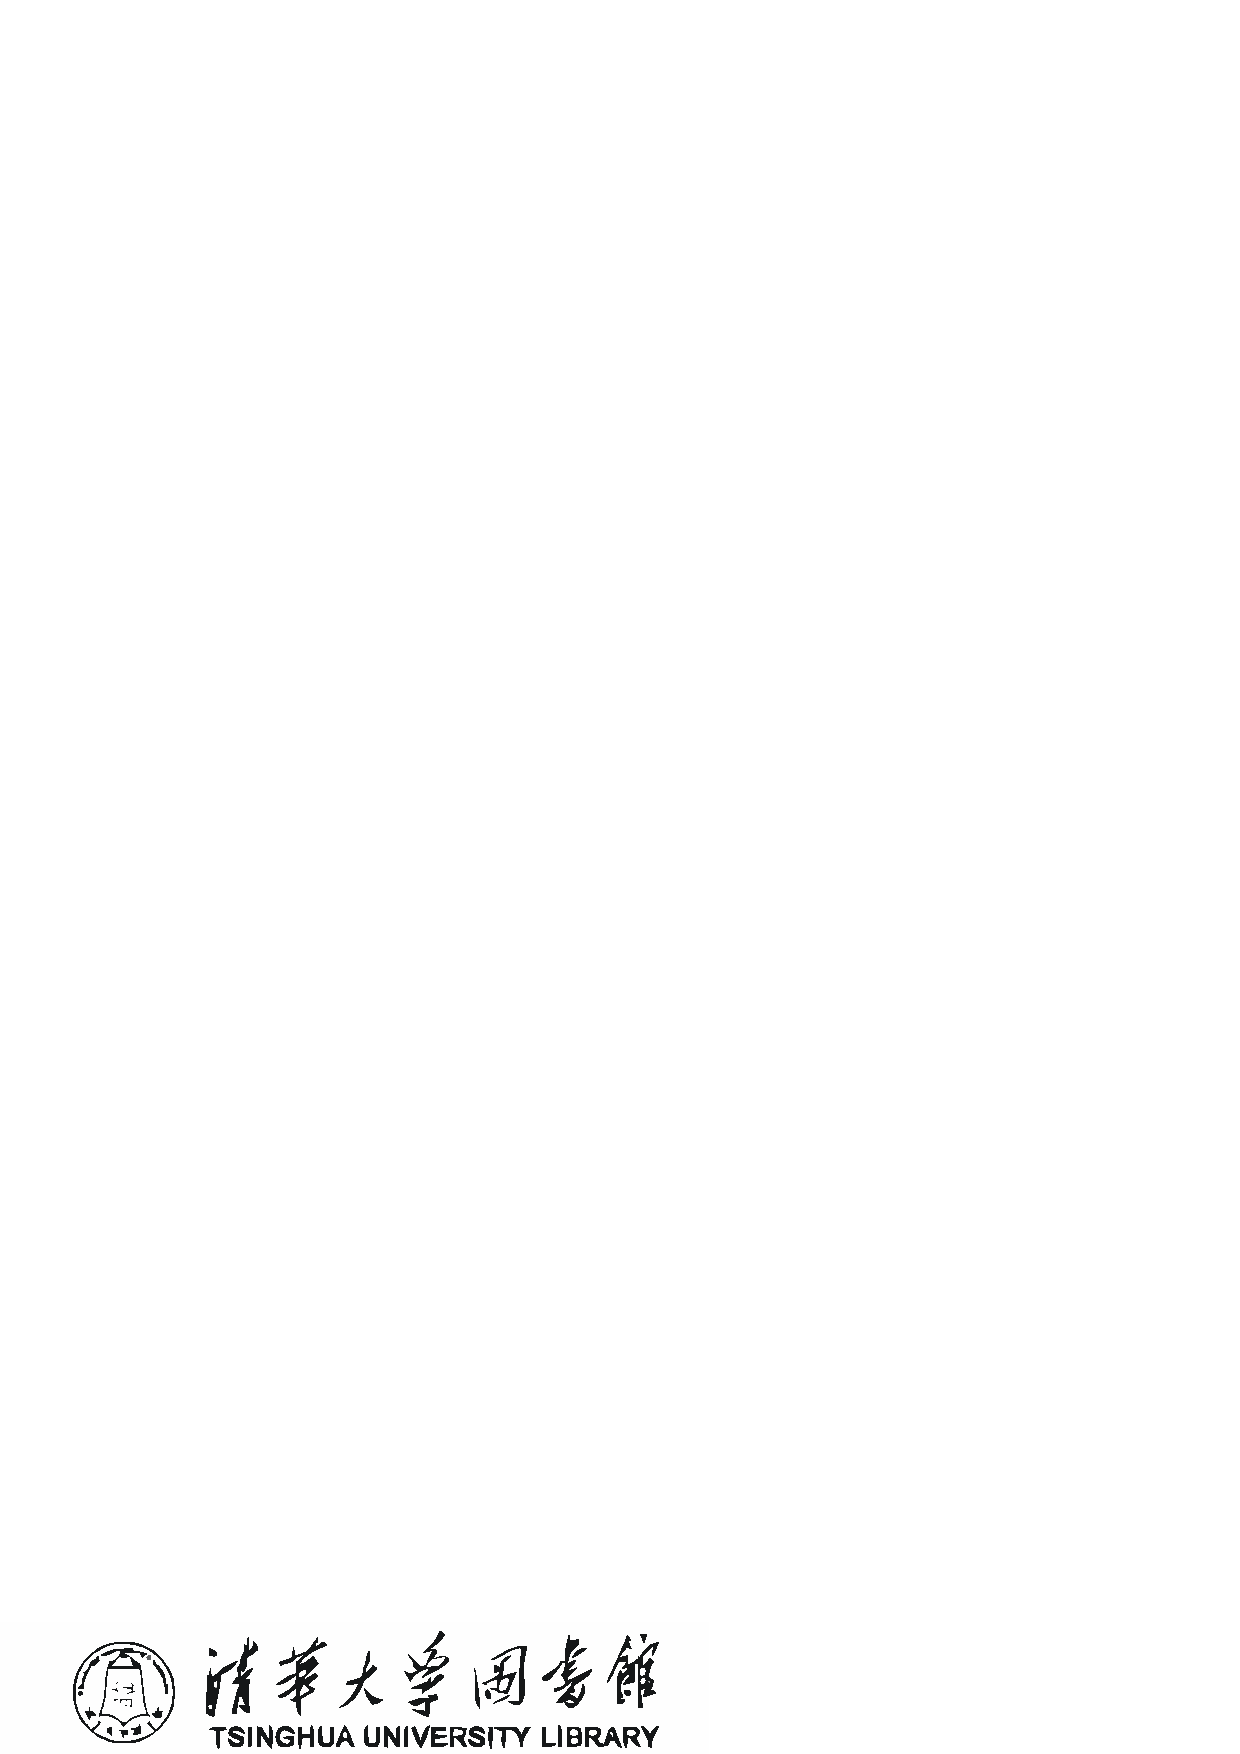
\includegraphics{thu-lib-logo}
  \caption*{Figure~1\quad This is an example for manually numbered figure,
    which would not appear in the list of figures}
  \label{tab:badfigure2}
\end{figure}

Now we consider a nonlinear programming which is confronted solely with
maximizing a real-valued function with domain $\Re^n$.  Whether derivatives are
available or not, the usual strategy is first to select a point in $\Re^n$ which
is thought to be the most likely place where the maximum exists. If there is no
information available on which to base such a selection, a point is chosen at
random. From this first point an attempt is made to construct a sequence of
points, each of which yields an improved objective function value over its
predecessor. The next point to be added to the sequence is chosen by analyzing
the behavior of the function at the previous points. This construction continues
until some termination criterion is met. Methods based upon this strategy are
called {\em ascent methods}, which can be classified as {\em direct methods},
{\em gradient methods}, and {\em Hessian methods} according to the information
about the behavior of objective function $f$. Direct methods require only that
the function can be evaluated at each point. Gradient methods require the
evaluation of first derivatives of $f$. Hessian methods require the evaluation
of second derivatives. In fact, there is no superior method for all
problems. The efficiency of a method is very much dependent upon the objective
function.

\subsection{Integer Programming}

{\em Integer programming} is a special mathematical programming in which all of
the variables are assumed to be only integer values. When there are not only
integer variables but also conventional continuous variables, we call it {\em
  mixed integer programming}. If all the variables are assumed either 0 or 1,
then the problem is termed a {\em zero-one programming}. Although integer
programming can be solved by an {\em exhaustive enumeration} theoretically, it
is impractical to solve realistically sized integer programming problems. The
most successful algorithm so far found to solve integer programming is called
the {\em branch-and-bound enumeration} developed by Balas (1965) and Dakin
(1965). The other technique to integer programming is the {\em cutting plane
  method} developed by Gomory (1959).

\hfill\textit{Uncertain Programming\/}\quad(\textsl{BaoDing Liu, 2006.2})

\section*{References}
\noindent{\itshape NOTE: These references are only for demonstration. They are
  not real citations in the original text.}

\begin{translationbib}
\item Donald E. Knuth. The \TeX book. Addison-Wesley, 1984. ISBN: 0-201-13448-9
\item Paul W. Abrahams, Karl Berry and Kathryn A. Hargreaves. \TeX\ for the
  Impatient. Addison-Wesley, 1990. ISBN: 0-201-51375-7
\item David Salomon. The advanced \TeX book.  New York : Springer, 1995. ISBN:0-387-94556-3
\end{translationbib}

\chapter{外文资料的调研阅读报告或书面翻译}

\title{英文资料的中文标题}

{\heiti 摘要:} 本章为外文资料翻译内容。如果有摘要可以直接写上来,这部分好像没有
明确的规定。

\section{单目标规划}
北冥有鱼,其名为鲲。鲲之大,不知其几千里也。化而为鸟,其名为鹏。鹏之背,不知其几
千里也。怒而飞,其翼若垂天之云。是鸟也,海运则将徙于南冥。南冥者,天池也。
\begin{equation}\tag*{(123)}
 p(y|\mathbf{x}) = \frac{p(\mathbf{x},y)}{p(\mathbf{x})}=
\frac{p(\mathbf{x}|y)p(y)}{p(\mathbf{x})}
\end{equation}

吾生也有涯,而知也无涯。以有涯随无涯,殆已!已而为知者,殆而已矣!为善无近名,为
恶无近刑,缘督以为经,可以保身,可以全生,可以养亲,可以尽年。

\subsection{线性规划}
庖丁为文惠君解牛,手之所触,肩之所倚,足之所履,膝之所倚,砉然响然,奏刀騞然,莫
不中音,合于桑林之舞,乃中经首之会。
\begin{table}[ht]
\centering
  \centering
  \caption*{表~1\hskip1em 这是手动编号但不出现在索引中的一个表格例子}
  \label{tab:badtabular3}
  \begin{tabular}[c]{|m{1.5cm}|c|c|c|c|c|c|}\hline
    \multicolumn{2}{|c|}{Network Topology} & \# of nodes &
    \multicolumn{3}{c|}{\# of clients} & Server \\\hline
    GT-ITM & Waxman Transit-Stub & 600 &
    \multirow{2}{2em}{2\%}&
    \multirow{2}{2em}{10\%}&
    \multirow{2}{2em}{50\%}&
    \multirow{2}{1.2in}{Max. Connectivity}\\\cline{1-3}
    \multicolumn{2}{|c|}{Inet-2.1} & 6000 & & & &\\\hline
    \multirow{2}{1.5cm}{Xue} & Rui  & Ni &\multicolumn{4}{c|}{\multirow{2}*{\thuthesis}}\\\cline{2-3}
    & \multicolumn{2}{c|}{ABCDEF} &\multicolumn{4}{c|}{} \\\hline
\end{tabular}
\end{table}

文惠君曰:“嘻,善哉!技盖至此乎?”庖丁释刀对曰:“臣之所好者道也,进乎技矣。始臣之
解牛之时,所见无非全牛者;三年之后,未尝见全牛也;方今之时,臣以神遇而不以目视,
官知止而神欲行。依乎天理,批大郤,导大窾,因其固然。技经肯綮之未尝,而况大坬乎!
良庖岁更刀,割也;族庖月更刀,折也;今臣之刀十九年矣,所解数千牛矣,而刀刃若新发
于硎。彼节者有间而刀刃者无厚,以无厚入有间,恢恢乎其于游刃必有余地矣。是以十九年
而刀刃若新发于硎。虽然,每至于族,吾见其难为,怵然为戒,视为止,行为迟,动刀甚微,
謋然已解,如土委地。提刀而立,为之而四顾,为之踌躇满志,善刀而藏之。”

文惠君曰:“善哉!吾闻庖丁之言,得养生焉。”


\subsection{非线性规划}
孔子与柳下季为友,柳下季之弟名曰盗跖。盗跖从卒九千人,横行天下,侵暴诸侯。穴室枢
户,驱人牛马,取人妇女。贪得忘亲,不顾父母兄弟,不祭先祖。所过之邑,大国守城,小
国入保,万民苦之。孔子谓柳下季曰:“夫为人父者,必能诏其子;为人兄者,必能教其弟。
若父不能诏其子,兄不能教其弟,则无贵父子兄弟之亲矣。今先生,世之才士也,弟为盗
跖,为天下害,而弗能教也,丘窃为先生羞之。丘请为先生往说之。”
\begin{figure}[h]
  \centering
  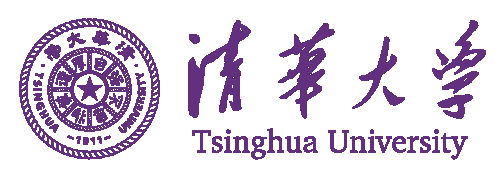
\includegraphics{thu-whole-logo}
  \caption*{图~1\hskip1em 这是手动编号但不出现索引中的图片的例子}
  \label{tab:badfigure3}
\end{figure}

柳下季曰:“先生言为人父者必能诏其子,为人兄者必能教其弟,若子不听父之诏,弟不受
兄之教,虽今先生之辩,将奈之何哉?且跖之为人也,心如涌泉,意如飘风,强足以距敌,
辩足以饰非。顺其心则喜,逆其心则怒,易辱人以言。先生必无往。”

孔子不听,颜回为驭,子贡为右,往见盗跖。

\subsection{整数规划}
盗跖乃方休卒徒大山之阳,脍人肝而餔之。孔子下车而前,见谒者曰:“鲁人孔丘,闻将军
高义,敬再拜谒者。”谒者入通。盗跖闻之大怒,目如明星,发上指冠,曰:“此夫鲁国之
巧伪人孔丘非邪?为我告之:尔作言造语,妄称文、武,冠枝木之冠,带死牛之胁,多辞缪
说,不耕而食,不织而衣,摇唇鼓舌,擅生是非,以迷天下之主,使天下学士不反其本,妄
作孝弟,而侥幸于封侯富贵者也。子之罪大极重,疾走归!不然,我将以子肝益昼餔之膳。”


\chapter{其它附录}
前面两个附录主要是给本科生做例子。其它附录的内容可以放到这里,当然如果你愿意,可
以把这部分也放到独立的文件中,然后将其 \cs{input} 到主文件中。

\end{appendix}

%% 个人简历
%\begin{resume}

  \resumeitem{个人简历}

  1991 年 03 月 01 日出生于 河北 邢台 市。

  2008 年 9 月考入 河北工业 大学  电气工程 系 电气工程及其自动化 专业,2012 年 6 月本科毕业并获得 工学 学士学位。

  2012 年 8 月免试进入 清华 大学 高等研究院 攻读 博士 学位至今。

  \researchitem{在学期间发表的学术论文} % 发表的和录用的合在一起
\noindent 1. 已经刊载的学术论文%(本人是第一作者,或者导师为第一作者本人是第二作者)

  \begin{publications}
  \item Xiaokai Huo, Wen-An Yong. Global existence for viscoelastic fluids with infinite Weissenberg number. Communications in Mathematical Sciences, 2017, 15(4): 1129-1140.(SCI收录)
  \item Xiaokai Huo, Wen-An Yong. Structural stability of a 1D compressible viscoelastic fluid model. Journal of Differential Equations, 2016, 261(2): 1264-1284.(SCI收录)
  \item Xiaokai Huo, Weitao Sun, et al. Coupling analysis of low-speed multiphase flow and high-frequency electromagnetic field in a complex pipeline structure. Mathematical Problems in Engineering, 2014(3):1-9.(SCI收录)
  \end{publications}

%  \noindent 2. 已经接收的学术论文%(本人是第一作者,或者导师为第一作者本人是第二作者)

 % \begin{publications}
%  \item Xiaokai Huo, Wen-An Yong. Global existence for viscoelastic fluids with infinite Weissenberg number. Communications in Mathematical Sciences, 2017, 15(229).(SCI收录)
  %\end{publications}

\end{resume}

\end{document}
